%4cm binding margin left
%2cm head margin top
%2.5cm fore-edge margin right
%4cm tail margin  bottom
%a4 is 21 x 29.7 cm

%1.5 spacing for main body, 
%single spacing for bibliography

%% Master tex file for the thesis.

%\documentclass[11pt,a4paper]{book} % double-sided
\documentclass[12pt,a4paper]{report}
\usepackage{subfigure,epsfig,amstext,floatfig,alltt,fancyhdr,setspace,xspace,amsmath,slashed,xfrac,amssymb}
\include{macros}
\initfloatingfigs

%%% helps to discourage hyphenation 10000 for no hyphens but dodgy line lengths%%%
\hyphenpenalty=5000
\tolerance=1000

% sets all the margins to be the correct size for thesis

%%%%%%% FINAL THESIS MARGINS  %%%%%%%%%
\setlength{\oddsidemargin}{0.7cm}
%\setlength{\evensidemargin}{1.46cm}
\setlength{\evensidemargin}{-0.04cm}
%\setlength{\evensidemargin}{0cm}
\setlength{\textwidth}{14.5cm}
\setlength{\topmargin}{-0.94cm}
\setlength{\textheight}{21.9cm} %22.2
\renewcommand{\hoffset}{0cm}
\renewcommand{\voffset}{0cm}
%%%%%%%%%%%%%%%%%%%%%%%%%%%%%%%%%%%%%%%



%% In the beginning ....
\begin{document}
%% First do introductory stuff - leave this as pagestyle empty until after
%% the table of contents
%\pagestyle{empty}
%
%\title{
\thispagestyle{plain}

\begin{center}
\LARGE
%\vspace*{2cm}
{\bf  Searching for SUSY in events with Jets and Missing Transverse Energy using $\alpha_{T}$ with the CMS Detector at the LHC}

\vspace{1cm}
%\begin{figure}[!ht]

\Large
{\it Zo\"e Hatherell}

\vspace{2cm}
\large
High Energy Physics Group\\
Department of Physics, Blackett Laboratory\\
Imperial College London\\
\vspace{2cm}

%\begin{center}        
A thesis submitted in fulfilment of\\
the requirements
for the degree of \\
Doctor of Philosophy\\
\vspace{1cm}

April 2012
\end{center}
%\maketitle     


%\ \newpage		% Newpage needed if doing double sided.



%% Include abstract - use separate parskip for this and then set parskip for
%% rest of thesis.
%\pagestyle{plain}

%-----------------------------------------------------------------------------

\pagestyle{fancy}
\fancyhead{} %clear all fields
\renewcommand{\headheight}{28pt}
\cfoot{}
\fancyfoot[LE,RO]{\thepage}

\renewcommand{\chaptermark}[1]{\markboth{\chaptername \ \thechapter.\ #1}{}} 
\renewcommand{\sectionmark}[1]{\markright{\thesection.\ #1} {}}

\fancyhead[LE]{\small \slshape \leftmark}      % Chapter in the right on even pages
\fancyhead[RO]{\small \slshape \rightmark}     % Section in the left on odd pages
\renewcommand{\headrulewidth}{0.3pt}    % Width of head rule

%-----------------------------------------------------------------------------


\pagenumbering{roman}
\setcounter{page}{1}
\newcommand\rs{\raisebox{1.0ex}[-1.0ex]}
\newcommand{\ra}{\ensuremath{\rightarrow}}
\newcommand{\HT}{\ensuremath{H_{T}}}
\newcommand{\znunu}{\ensuremath{{\text Z} \ra \nu\bar{\nu}}}
\newcommand{\zmumu}{\ensuremath{{\text Z} \ra \mu\mu}}
\newcommand{\wmunu}{\ensuremath{{\text W} \ra \mu\nu}}
\newcommand{\wtaunu}{\ensuremath{{\text W} \ra \tau\nu}}
\newcommand{\dphi}{\ensuremath{\Delta \phi}}
\newcommand{\dphijj}{\ensuremath{\Delta \phi_{ j1,j2}}}
\newcommand{\Pt}{\ensuremath{{p_{\text T}}\xspace}}
\newcommand{\pts}{\ensuremath{p_{\text T}{\text s}}\xspace}
\newcommand{\Et}{\ensuremath{{E_{\text T}}\xspace}}
\newcommand{\ptjf}{\ensuremath{p_{\rm T}^{ {\rm j}_1} }}
\newcommand{\ptjs}{\ensuremath{p_{\rm T}^{ {\rm j}_2} }}
\newcommand{\ptjt}{\ensuremath{p_{\rm T}^{ {\rm j}_3} }}
\newcommand{\etajf}{\ensuremath{\eta^{ {\rm j}_1} }}
\newcommand{\etajs}{\ensuremath{\eta^{ {\rm j}_2} }}
\newcommand{\etajt}{\ensuremath{\eta^{ {\rm j}_3} }}
\newcommand{\ttj}{\ensuremath{\rm{t}\bar{\rm{t}} + jets}\xspace}
\newcommand{\wj}{\ensuremath{\rm W + jets}\xspace}
\newcommand{\zj}{\ensuremath{\rm Z + jets}\xspace}
\newcommand{\al}{\ensuremath{\alpha}}
\newcommand{\alt}{\ensuremath{\alpha_{\text{T}}}\xspace}
\newcommand{\etaabs}{\ensuremath{|\eta|}}
%\newcommand{\gev}{\ensuremath{\mathrm{\,Ge\kern -0.1em V}}}
\newcommand{\pb}{\ensuremath{pb^{-1}}}
\newcommand{\mjj}{\ensuremath{M_{\text{inv}}^{j1,j2}}}
%\newcommand{\ttbar}{\ensuremath{t\bar{t}}}
\newcommand{\chiznew}{\ensuremath{\chi^{0}}\xspace}
\newcommand{\chipnew}{\ensuremath{\chi^{+}}\xspace}
\newcommand{\sQuanew}{\ensuremath{\tilde{\rm q}}\xspace}
\newcommand{\sGlunew}{\ensuremath{\tilde{\rm g}}\xspace}
\newcommand{\ttNew}{\ensuremath{\rm{t}\bar{\rm{t}}}\xspace}
\newcommand{\tev}{\TeV}
%<TW date="30/10/2010">
%\newcommand{\Et}{E_{T}}
\newcommand{\combIso}{Iso_{\textrm{comb.}}}
\renewcommand{\arraystretch}{1.2}
\newcommand{\bigNum}[2]{#1 \, \times \, 10 \, ^{#2}}
%</TW>

\newcommand{\raT}{\ensuremath{R_{\alt}}}
\newcommand{\RaT}{\ensuremath{R_{\alt}}\xspace}
\newcommand{\GeV}{\textrm{GeV}}
\def\eslash{{\hbox{$E$\kern-0.6em\lower-.05ex\hbox{/}\kern0.10em}}}
\def\vecmet{\mbox{$\vec{\eslash}_T$}} %missing ET vector
\def\vecet{\mbox{$\vec{E}_\text{T}$}} % ET vector
\def\MET{\mbox{$\eslash_\text{T}$}\xspace}
\def\met{\mbox{$\eslash_\text{T}$}\xspace}
\def\mex{\mbox{$\eslash_\text{x}$}} %missing Ex
\def\mey{\mbox{$\eslash_\text{y}$}} %missing Ey
\def\mepar{\mbox{$\eslash_\parallel$}}
\def\meperp{\mbox{$\eslash_\perp$}}
\def\Zmm{Z \rightarrow \mu\mu}
\def\metvec{\mbox{$\vec{\met}$}\xspace}
\def\metvecrec{\mbox{$\vec{\met}^{\rm rec}$}\xspace}
\def\metvecgen{\mbox{$\vec{\met}^{\rm gen}$}\xspace}
\def\metgen{\mbox{$\met^{\rm gen}$}\xspace}
\def\metparl{\mbox{$\mepar^{\rm rec}$}\xspace}
\def\metperp{\mbox{$\meperp^{\rm rec}$}\xspace}
\def\deltamet{\mbox{$\Delta\met$}\xspace}
\def\pthat{\mbox{$\hat{p}_T$}\xspace}
\def\hslash{{\hbox{$H$\kern-0.8em\lower-.05ex\hbox{/}\kern0.10em}}}
\def\MHT{\mbox{$\hslash_\text{T}$}\xspace}
\def\mht{\mbox{$\hslash_\text{T}$}\xspace}
\def\sumet{\mbox{$\sum \rm{E}_\text{T}$}\xspace}
\def\scalht{\mbox{$H_\text{T}$}\xspace}
\def\etmiss{\mbox{$\eslash_\text{T}$}\xspace}
\def\htmiss{\mbox{$\hslash_\text{T}$}\xspace}
\def\mtt{\mbox{$\rm{M}_\text{T2}$}\xspace}
\def\rmec{\mbox{$R_{\mht/\met}$}\xspace}
\def\bdphi{\mbox{$\Delta\phi^{*}$}\xspace}
\def\bigeslash{{\hbox{$E$\kern-0.38em\lower-.05ex\hbox{/}\kern0.10em}}}
\def\bigmet{\mbox{$\bigeslash_T$}}
\def\bighslash{{\hbox{$H$\kern-0.6em\lower-.05ex\hbox{/}\kern0.10em}}}
\def\bigmht{\mbox{$\bighslash_T$}}
\def\cls{\mbox{CL$_s$}\xspace}
\def\incl{\includegraphics[width=0.49\linewidth]}
\def\inclrot{\includegraphics[angle=90,width=0.47\linewidth]}
\def\INCL{\includegraphics[angle=90,width=0.45\linewidth]}
\def\Incl{\includegraphics[angle=90,width=0.60\linewidth]}




\onehalfspacing

%%\addcontentsline{toc}{chapter}{Abstract}
%\chapter*{Abstract}
\noindent 
\vspace{10mm}
\normalsize

A search for new physics resulting in missing energy in events with high \Pt jets is presented. The analysis is performed with 1.1fb$^{-1}$ of 7~TeV data taken using the Compact Muon Solenoid detector at the Large Hadron Collider in 2011.The kinematic variable \alt is used to control the background from fake missing energy originating from mis-measurment. The remaining electroweak backgrounds are estimated using data-driven techniques through the use of control samples. The background from boosted W decays is estimated with the use of a dedicated $\mu$ + jets control sample, while the irreducible background from Z $\ra \nu \bar{\nu}$ is estimated using a $\gamma$ + jets control sample.  A shape analysis is performed across 8 bins in \HT, with the signal selection alongside the two control samples are treated simultaneously in a likelihood fit.  The data was found to agree very well with the Standard Model only hypothesis with a p-value of 0.56, indicating no evidence of new physics. The results are interpreted in the scope of a popular new physics model, the Constrained Minimal Supersymmetric Standard Model. Exclusion limits are set at the 95\% confidence level on the parameters m$_{0}$ and m$_{1/2}$ that set the mass hierarchies of the sparticles. An extension is also presented allowing additional signal into the muon control sample. The effect on the limit is negligible, although adopting a leptonic variable of the \alt variable increases the ratio between signal and background events significantly. We recommend this approach in searches with higher statistics in 2012. 





%\ \newpage		% Newpage needed if printing double sided.

%\addcontentsline{toc}{chapter}{Declaration}
%\chapter*{Declaration}

\normalsize

The research undertaken in this thesis was the unaided work of the author, except where the work was done in collaboration
with others as indicated in the text. In this case a significant contribution was made by the author. All other work is referenced properly throughout the text. 

The analysis detailed in Chapter~\ref{ch:ra1} was performed by a small collaboration of which the author was a key member and made a significant contribution, including full responsibility for the muon control sample. The author's own personally conducted extension to the analysis is documented in Chapter~\ref{ch:ra4}. 





\vspace{20mm}
\hfill {\it Z. Hatherell}

\hfill March 2012







%\ \newpage		% Newpage needed if printing double sided.

\addcontentsline{toc}{chapter}{Acknowledgements}
%\chapter*{Acknowledgements}

%\noindent

\normalsize

I would like to extend my thanks to everyone who worked with me and helped me in the course of this Ph.D. I am sincerely and heartily grateful to my advisor, Jordan Nash, for the support and guidance he showed me throughout my time at Imperial College.

It has been a pleasure to be a member of the Imperial RA1 team alongside Rob Bainbridge, Burt Betchart, Oliver Buchm\"uller, Darren Burton, Edward Laird, Bryn Mathias, Henning Fl\"acher,Tanja Rommerskirchen, Paris Sphicas, Markus Stoye, and Tom Whyntie. It would also not have been possible without Georgia Karapostoli, for teaching me so much in the beginning. 



To all the wonderful UK LTA crew who are too numerous to name individually. Collectively you made my time at CERN the best time of my life and I one I will never forget. Special thanks to the LTA ladies for girly nights! 

To my parents Jan and Adrian, who have supported me through everything I have been through for my whole life and taught me that anything is within my grasp. Thanks for always believing in me and being there when the times were toughest. 

To Chris, for loving me. You 



\singlespacing

%\ \newpage		% Newpage needed if printing double sided.

%\addcontentsline{toc}{chapter}{Contents}
%\tableofcontents

%\ \newpage		% Newpage needed if printing double sided.
%\ \newpage		% Newpage needed if printing double sided.

%%%%%ZOE%\addcontentsline{toc}{chapter}{List of figures}
%%%ZOE\listoffigures

%\ \newpage		% Newpage needed if printing double sided.

%%%%ZOE\addcontentsline{toc}{chapter}{List of tables}
%%%%ZOE\listoftables
  
%\ \newpage		% Newpage needed if printing double sided.
%\ \newpage		% Newpage needed if printing double sided.

%%%ZOE\clearpage % this command stops table page becoming page 1


%% Now the body of the text - note that parskip has to be reset after the TOC

\onehalfspacing
\pagenumbering{arabic}

\setcounter{page}{1}
%% Add chapters here %%
%\setcounter{equation}{0}
\setcounter{figure}{0}
\setcounter{table}{0}

\chapter{\label{chapter1} Introduction}

Describe storyline of Thesis. 

%\section{Pressure as a Thermodynamic Variable}

%\section{Present Work and Thesis Outline}


\chapter{Theoretical Overview}

At the heart of particle physics is a quest to discover the fundamental building blocks of the universe, and how they interact with one another. The field is often given the alternative title "High Energy" physics, as the quest to investigate ever smaller distances as we zoom into the structure of our world is analogous to an increase in the energy scale necessary to view it. Throughout the history knowledge has been advanced through a combination of theoretical postulation using mathematical tools, and experimental searches. Particle physicists seek together to build a full description of the dynamics of the fundamental particles, and while they have discovered much, the picture is not complete yet. The current state of play is collectively known as the Standard Model (SM), and is a rigourously tested and widely accepted theory. However, whilst there are no disagreements, there are some gaps which hint at physics beyond, fuelling a new generation of experimentalists seeking answers to what lies behind.

\section{The Standard Model}

The Standard Model (SM) is the name given to the theories that successfully describes the known elementary particles and their fundamental interactions with respect to the strong, weak and electromagnetic forces.  These theories are formulated mathematically using quantum field theory (QFT), in which particles are thought of as excitations of fields, and the dynamics of a given system are summarised in a function called a Lagrangian. In order to reflect the symmetries observed in nature, measurements of physical properties in the SM must be invariant under local transformations, and this property is called gauge invariance. Therefore the SM is a special case of field theory, called Gauge Theory, and the interactions between particles are described by force-carrying mediation particles known as gauge bosons. From Noether's Theorem, it is known that as a consequence of a symmetry in a dynamical system there is an associated physically conserved quantity. Clearly, for the electromagnetic force this is the electric charge. Analogously, there are conserved "charges" for the strong and weak forces, "colour" charge and the quantum number "isospin", $T_{3}$ respectively. 
 
The set of possible transformations is described in the language of Group Theory, and thus we describe the SM as a non-Abelian Yang-Mills type gauge field theory based on the symmetry group $SU(3)_{C} \times SU(2)_{L} \times U(1)_{Y}$. The strong interactions described by Quantum Chromodynamics (QCD) are represented by $SU(3)_{C}$, and the electromagnetic and weak interactions are represented together due to Electroweak Unification by the group $SU(2)_L \times U(1)_{Y}$. As of yet, the fourth fundamental force Gravity is not included in the Standard Model, but this is seen as of little consequence as gravitational forces are thought to have comparatively little effect on fundamental particles. 


There exist two main types of fundamental particle, which in order to distinguish we must address the concept of spin. 
\begin{description}
\item[Spin] \hfill \\
Spin is the name given to a property of elementary particles, corresponding to a type of angular momentum, although this differs from classical angular momentum. This is an intrinsic property and thus has a specific value for each particle type. The values of the spin quantum number s which describe the magnitude can take any half integer value $s=0, \frac{1}{2}, 1, \frac{3}{2}$, etc. In addition to magnitude we describe a particle as having spin \textit{up} when the spin is in the direction of the z-axis, and spin \textit{down} if the spin is against the direction of the z-axis. When the spin direction is in the direction of momentum of the particle, it is described as left-handed, and when it is against as right-handed. 
\end{description}
All fundamental particles are divided into the spin-1/2 \textit{fermions} which are the building blocks for matter, and the force-mediating \textit{bosons} which must carry integer spin, usually spin-1. 
 

The fermions which make up all visible matter can be described in three families, or "generations", shown in Equation \ref{eqn:threefams}. Within each generation, there are two sets of particles, those on the left are the leptons, which interact by the weak and electromagnetic forces only, and those on the right are the quarks, which also interact by the strong force. In each generation, there are two quarks, which differ by electoral charge - one has +2/3 and the other -1/3 (in units of the electron charge \textit{e}), an electrically charged lepton and a neutral lepton called a neutrino which is either massless or very light. The three families then are organised in ascending order of mass. The first generation is therefore stable and all ordinary matter is constructed from it, whilst the second and third are liable to decay into particles of the first generation. In addition to each particle detailed here there exists a corresponding antiparticle due to a symmetry in charge and quantum numbers.  

\begin{equation}
\begin{bmatrix}
\nu_{e} & u \\
e & d \\
\end{bmatrix},
\begin{bmatrix}
\nu_{\mu} & c \\
\mu & s \\
\end{bmatrix},
\begin{bmatrix}
\nu_{\tau} & t \\
\tau & b\\
\end{bmatrix}
\label{eqn:threefams}
\end{equation}

The particles which mediate the forces are bosons, the photon $\gamma$ for the electromagnetic force, the 8 gluons $g_{i}$ for the strong force and the $W^{\pm}$ and Z bosons that carry the Weak force, all of which are spin-1 particles. The final particle of the SM is the Higgs Boson of spin-0, as yet undiscovered in experiment but expected from the theory, as we will see later. 

\subsection{Gauge Theory of Interactions}

Everything in our Universe interacts by way of gauge bosons mediating one of the four fundamental forces. Whilst the SM incorporates the electromagnetic, strong and weak forces, it as of yet has not been possible to describe the gravitational force in this way. 


\subsubsection{Quantum ElectroDynamics}

The fundamental electromagnetic force is studied in quantum field theory as Quantum Electrodynamics (QED), the oldest and simplest of the theories brought together to form the SM. The symmetry of QED is U(1) and this gives an associated conserved quantity, the electric charge Q. The electromagnetic force is carried by the massless boson, the photon, and affects only the charged fermions. The symmetry allows no self interaction of the photon. The fermion field $\psi_{q}$ with charge $q$ and mass $m_{q}$ gives rise to the Lagrangian in Equation \ref{eqn:QEDL}. 

Lagrangian 
\begin{equation}
\Lagr_{QED} = \bar{\psi}_{q}(i \gamma^{\mu}\slashed{D}_{QED,\mu} - m_{q}) \psi_{q} - \frac{1}{4}F_{\mu \nu}F^{\mu \nu}
\label{eqn:QEDL}
\end{equation}

Here, $\slashed{D}_{QED,\mu}$is the covariant derivative, incorporating the introduction of a photon gauge field $A_{\mu}$, so as to maintain an invariance to local U(1) charge symmetry. Thus, 
\begin{equation}
\slashed{D}_{QED,\mu} = \partial_{\mu} + iQA_{\mu}
\end{equation}
where Q is described as the generator of the symmetry group and is analogous to electric charge. The strength of coupling of each force is described by the coupling constant, in this case governed by the constant e, the charge of an electron: $\alpha = \frac{e^{2}}{4\pi}$ 

\subsubsection{QCD}

Quantum Chromodynamics (QCD) is the relevant quantum field theory that describes the dynamics of the strong force. The strong force of symmetry group $SU(3)_{C}$ has 8 massless gauge bosons known as the gluons, and a conserved quantity called colour charge, which has three types called $q_{i} i=1,2,3$. The name "colour" is not meant to imply a connection to visual colour, merely an analogy between the three types and the primary colours red, blue and green. Only particles which carry colour charge are affected - the quarks have colour, while leptons do not. Unlike the photon in electromagnetism, the gluons that mediate the force carry the charge also, leading to the self-interactions that govern the behaviour of QCD. 

A quark carries one "colour" $q_{i}$, taking one of the three possible values, and an analogous antiquark carries one "anti-colour". On the other hand, gluons carry both a colour and an anti-colour.  Separation of two charges gives rise to a potential energy, which increases linearly as the charges are moved further apart. As a consequence, it would take an infinite amount of energy to separate two quarks, and thus they are not found free in nature, but only bound within colourless hadrons such as the proton p $\sim$ uud and the neutron n $\sim$ dud, an effect we call \textit{confinement}. This explains why colour charge is not observed in nature, as beyond a fundamental level it has no meaning.

 To describe this behaviour, the coupling constant of the strong force, $\alpha_{S}$  as the distance between two particles is increased, or as the energy scale is increased, in comparison to the coupling constant for QED which has the inverse relationship. When we discuss quarks in particle physics although they are free, this is as a result of the "asymptotic freedom" where when viewed at very large energies the distances are infinitely small, and the quarks behave freely. tat

\begin{equation}
\Lagr_{QCD} = \sum_{q} \bar{q}(i \gamma^{\mu}\slashed{D}_{QCD,\mu} - m_{q}) q - \frac{1}{4}F^{\alpha}_{\mu \nu}F^{\mu \nu}_{\alpha}
\label{eqn:QCDL}
\end{equation}



\subsubsection{The Weak Force and Electroweak Unification}

The weak interaction, responsible for radioactive decay, makes up the final piece of the puzzle. So named because of its comparatively low strength compared to the electromagnetic and strong forces, it is was theorised as being mediated by massive force bosons $W^{\pm}$ and Z long before they were discovered experimentally. A lagrangian theory for the weak force must take into account the characteristics of weak interactions. Firstly, it is capable of flavour changing in quark interactions. Secondly, it shows a chirality whereby it interacts with only left-handed fermions, and right handed anti-fermions, violating Parity, P. It also violates ye Thirdly it is capable of both charged interactions which violate the charge C, and neutral interactions which do not. Whilst C and P can both be violated, the product CP 

 describing the interactions of the left-handed fermion doublets. The group symmetry is SU(2) giving rise to a conserved quantity known as weak isospin, I. Building an individual Lagrangian to describe the picture of weak interactions was not as simple as in the strong and electromagnetic sectors, with each proposed model suffering problems. Finally it was realised that despite their apparent differences the weak and electromagnetic forces were low-energy manifestations of the same force, and a composite theory was proposed~\cite{Glashow}. This is called Electroweak Unification, and for this the Nobel Prize was awarded to Glashow, Salam and Weinberg in 1979~\cite{Breaking}. 

The gauge group of the unified theory is $SU(2)_{L} \times U(1)_{Y}$, where $U(1)_{Y}$ is a different copy of the symmetry seen in electromagnetism, the $U(1)_{em}$ group. In this picture the conserved quantity is Y, the weak hypercharge, and the conserved quantity for the SU(2) symmetry is the weak isospin, $T_{3}$. The previous quantity conserved under $U(1)_{em}$ Q can be defined as a linear combination of the two $Q = T_{3} + \frac{Y}{2}$.  The $SU(2)_{L}$ suffix is not taken from the conserved quantity, $T_{3}$, but from it most important property, its action on only Left Handed (LH) fermions. Fermions that are Right Handed (RH) have a weak isospin $T_{3} = 0$ and do not interact via the weak force, whereas LH fermions have $T_{3} =  \pm \frac{1}{2}$ and interact via three gauge bosons. The $W^{\pm}$ bosons have each an isospin of unit 1, with a sign defined by the name, and they govern an interaction from a particle of $T_{3}=+\frac{1}{2}$ into one of $T_{3}=-\frac{1}{2}$ and vice versa, according to conservation laws. The third boson given by the SU(2) group alone is the $W^{0}$ boson of $T_{3}=0$, which allows interactions where the weak isospin stays the same. This is not a physically observed particle, as the electroweak unification leads to mixing between this and the boson given by the $U(1)_{Y}$ group to produce the photon and the $Z^{0}$ particle. 

\subsection{EWSB and the Higgs Mechanism}

In order to give mass to the W and Z bosons whilst retaining the necessary local gauge invariance, we say that $SU(2)_{L} \times U(1)_{Y}$ must be spontaneously broken into $U(1)_{em}$, the group of symmetries representing the electromagnetic sector. The simplest way to introduce such a breaking is known as the Higgs Mechanism, and corresponds to the addition of a scalar field. Ensuring the change to the Lagrangian is invariant, there is a covariant derivative term and an additional potential. With the construction of a potential colloquially known as a "mexican hat" potential [NEEDPIC], the minimum does not lie at $\phi$ = 0, but in 3D space in a circle of minima around $\phi$, so there are an infinite number of minima, introducing a degeneracy. As a particular vacuum is chosen, the symmetry is broken. Interactions with the field lead to masses for the W and Z bosons. This leads to the existence of a massive scalar particle, known as the Higgs Boson, to date the only particle of the SM yet to be observed. 

The distinction between the two forces caused by this symmetry breaking are due to a linear combination of the weak hyper charge and isospin, $T_{3}$ and Y that vanishes for the Higgs. As this defines the conserved quantity Q for the electromagnetic group, this is not affected by the higgs, and thus the $U(1)_{em}$ group remains unbroken. Conversely, the weak portion interacts with the Higgs and the W$\pm$ and Z bosons acquire mass.  

\section{Motivation for Physics Beyond the Standard Model}
The standard model has been widely successful, predicting the existence of particles such as the $W^{\pm}$ and Z Bosons, and the t quark, showing impressive agreement with experimental findings at the level of 0.1\%. However, there are several signs that it is not a complete theory, that more information is needed to describe physics at higher energy scales. It can be assumed that the Standard Model is a low-energy . 

The SM does not currently incorporate the gravitational force, a problem which has not bothered particle physicists much as the strength of the effects of gravity on fundamental particles is negligible compared to the other fundamental forces. However, at an energy known as the Plank Scale, $M_{p} \sim 1-^{18}$ GeV quantum gravitational effects become important, leading to the breakdown of the existing QFT picture of the Standard Model. Thus new physics must exist at this energy scale, or before, indicating the SM is only valid up to some unknown energy scale. Several other theoretical problems exist motivating theories for physics Beyond the Standard Model (BSM) at the TeV scale, which we are able to explore for the first time with the LHC. 

 nor does it explain the existence of dark matter and dark energy. Neutrino masses and flavour mixing are also unexplained. In addition, several features of the existing SM are seen as inelegant, as they require some mathematical fine-tuning and thus are unlikely to reflect nature. The main motivations for 
\subsection{The Hierarchy Problem}

Although the Higgs Boson has yet to be observed experimentally, its mechanism is necessary to the Standard Model to provide mass to the particles, and thus is considered to exist unless proven otherwise. However, while it solves the SSB problem, the Higgs theory introduces theoretical issues of its own. The presence of the Higgs in the SM ensures the WW scattering amplitude does not violate unitarity, but only whilst the $m_{H} < 1 TeV$, providing an upper bound on the expected mass\cite{WWHMass}. 

However, in the coupling of the Higgs to heavy fermions, the mass of the Higgs receives extremely large radiative corrections. If each coupling with a fermion f has a term in the Lagrangian $-\lambda_{F} H \bar{f}f$, it contributes a quadratically divergent factor $\delta m^{2}_{H}$ that corrects the squared mass of the Higgs. 

\begin{equation}
\delta m^{2}_{H} = - \frac{|\lambda_{f}|^{2}|}{8 \pi^{2}}\Lambda^{2}_{UV}
\label{eqn:HIGGQUAD}
\end{equation}

The parameter $\Lambda_{UV}$ is the \textit{ultraviolet cutoff}, so named as it represents the smallest distance to probe in the calculation. It can be thought of as the scale at which the Standard Model is valid up to, as any new physics would change the theory. If there were no new physics at a lower energy, it takes the value of the Plank Scale $M_{P}$, but in this case the correction will be 30 orders of magnitude higher than the 1 TeV upper bound justified experimentally. As there exists nothing in the SM to fix the Higgs Mass, the theory requires fine-tuning, tweaking the parameters to agree with observational findings. This is generally accepted to be an inelegant method, as it requires the input of extra information, and indicates a gap in the fundamental description leading to searches for extensions to the Standard Model. 

\subsection{Cold Dark Matter}

The existence of Dark Matter was postulated as early as 1933 by Zwicky \cite{zwicky}, as the orbital velocities of galaxies in clusters were inconsistent with their observed mass, suggesting some additional mass was present but not luminous.  Measurments of rotation curves of galaxies, cosmic microwave background and structure formation have confirmed this concept over the years. Experimental results from WMAP conclude only $\sim 4.5\%$ of the energy in our universe is made of the baryonic matter we see, while dark matter accounts for $\sim 23\%$ and the rest is comprised of another unknown, dark energy. Although the existence of such matter has been well documented, there is still no understanding of the physics behind the phenomena. In order to explain the properties a weakly interacting massive particle (WIMP) is required, and it must be electrically neutral. There is no provisions for such a particle in the SM, indicating additional particle content requiring extensions in the theory. 

\subsection{Unification of Coupling Constants}

At the basis of theoretical particle physics is the observation of the symmetry and simplicity of nature. Unification, where several theories can be combined into one description,  has undergone before, first Electricity and magnetism, and then electromagnetism with the weak force. While each of the three forces of the SM have their own coupling constant, as the energy scale is increased the coupling constants converge towards one another. However precision measurements show that within the current framework,  there is no common point where all three intersect. In addition, at the Planck Scale as gravity's coupling constant would be of similar strength many hope for a Grand Unified Theory (GUT),  occurring at this scale known also as the GUT scale. This is only possible with the incorporation of some new physics which would alter the trend of the couplings between the electroweak scale and this GUT scale. 


\section{Supersymmetry}

The hierarchy problem could be removed, rather than controlled, if there were a way to cancel out the quadratic diverging term in the Higgs mass correction. As the correction for bosons has the opposite sign, the conception of a new symmetry was born, one between fermions and bosons. Known as SUperSYmmetry (SUSY), this theory extends the SM under this symmetry such that elementary particles in the SM each have a super partner differing by one half unit of spin as yet undiscovered, just as the anti-particles were once postulated. For every fermion contributing to the quadratic divergence, a boson partner contributes the equal and opposite term, and thus the hierarchy problem cancels out and the mass of the higgs can take a sensible value.

Under this symmetry elementary particles in the SM would each have corresponding super-partners, differing by one half unit of spin, such that a fermion has a scalar boson super partner, and vice versa. At the heart of supersymmetry is a transformation that changes the field of a fermion into that of a boson, and vice versa. The generator of the transformation shall be known as Q,

\begin{equation}
Q|fermion> = |boson>, 	Q|boson> = |fermion> 
\label{eqn:Q}
\end{equation}

According to an exact symmetry a super partner would have the same characteristics as its partner, including its mass, which would indicate they were within the reach of previous physics experiments. However, they have not been observed, and thus it is concluded that the symmetry is broken at some energy scale, to give the superpartners greater mass. In order for SUSY to eliminate the hierarchy problem, this breaking is assumed to occur at the Electroweak Scale, which restricts the size of the difference in mass to the order of ~1 TeV.  This is known as "soft" SUSY breaking, and offers the hope of discovering this new physics at the TeV scale, as is now possible for the first time with the LHC. 

In addition to its neat solution to the hierarchy problem SUSY has several other consequences which lead to its position as the most favoured theory for new physics at the TeV scale. The inclusion of SUSY particles to the SM has the side affect of altering the runnings of the gauge coupling constants of the three fundamental forces, discussed above, such that they are consistent with theories of Grand Unification, an energy scale at which the three are equal. Rather than a motivation, this is a pleasant coincidence, but lends plausibility to the theory. It also shows promising features necessary for theories to incorporate gravity, although it does not finish the job. SUSY itself cannot be the final fundamental theory of particle physics, but is an extension which shows much promise. The final, perhaps most exciting feature of SUSY is that it can offer a candidate for the particle that represents dark matterm with the introduction of a new quantum number R - Parity. 



\subsection{R-Parity}

Consructing the most general form of SUSY, terms appear which allow processes which violate two quantum numbers, the baryon number B and the lepton number L. Whilst there is no theoretical reason for this to be a problem, these interactions have not been observed, and are constrained heavily. An undeniable constraint is the lifetime of the proton, which is very large, whereas these processes would facilitate its decay. whilst B and L are not fundamental symmetries in the theory, it is possible to construct a new quantum number R defined in Equation \ref{eqn:RPAR} which can be required as a symmetry R-parity. It distinguishes between particles from the SM and the sparticles introduced by SUSY, as under this construction, all SM particles carry $R$ of +1 and all super partners carry -1. 

\begin{equation}
R = (-1)^{3(B-L)+2S}
\label{eqn:RPAR}
\end{equation}
Whilst terms in the Quantum Field Theory do allow for the possibility of violation of this parity, experimental measurements has excluded this for sparticles with masses on the TeV scale, and therefore those within the reach of the LHC. Thus the  majority of searches consider models with a symmetry which forbids this violation and conserves Rp. Several phenomenological consequences arise from this assumption which provide the backbone to SUSY searches at the LHC. 

IN over for SUSY particles to be produced at the LHC under this framework, they must be pair produced from SM particles. The heavier particles undergo a decay chain ending in the lightest of the supersymmetric particles, denoted the Lightest Super Partner (LSP), and this particle is by necessity stable and neutral, as it cannot decay into SM particles. These characteristics denote it a WIMP, the type of particle that is sought in Dark Matter searches.  These particles will not interact in a detector, therefore are characterised in an experiment as large amounts of missing energy. As this is directly a characteristic of a WIMP in the final state, such a signature represents not only SUSY but is shared by other new physics models with a dark matter candidate particle. 

Models may be constructed to constrain the violation of B and L without R-parity conservation, but those shall not be considered in this thesis, as this unique feature provides both physical motivation and a search strategy for physics at the LHC.


\subsection{MSSM} 

Whilst there are money ways to construct mathematically the theory of Supersymmery, it is usual to do it in the way which introduces the least number of new degrees of freedom. This corresponds to the minimal particle contact required to satisfy the core symmetry, which corresponds to one new degree of freedom for each existing SM one. This approach is known as the Minimal Supersymetric Standard Model (MSSM), and has an additional new particles, known as a sparticle, for each known SM particle. 

The particles are arranged to fit the irreducible representation of the symmetry, in \textit{supermultiplets}, each of which contains both fermions and bosons. The number of bosonic and sermonic degrees of freedom are therefore equal in any supermultiplet. The names of the spin-0 bosons that partner the SM fermions are prepended by "s", known as squarks and sleptons, collectively the sfermions. 

The Higgs receives different treatment in SUSY, as not one but two Higgs supermutiplets are required, to give mass separately to the quarks of charge \sfrac{1}{3} and the quarks of charge \sfrac{2}{3}



\subsection{Minimal Supergravity and the Constrained MSSM}

Even assuming a minimal particle content, the MSSM has a large number of free parameters, introduced through SUSY and Electroweak symmetry breaking, 105 more than the SM. When it comes to experimental searches, this is an unworkable number, for to examine possible behaviour of SUSY one would have to look in 105 dimensions. Thus for the purpose of making models to work with, it is desired to constrain this number in the theory. One popular theory used in this thesis is the theory of minimal SUper GRAvity, otherwise known as mSUGRA. 

The concept behind mSUGRA is that there should be some messenger between the MSMM sector and 

\subsubsection{Current Limits on the CMSSM}

Two types of limits exist in mSUGRA space, those imposed theoretically and those that result from experimental data. Of the latter, some are contributed from cosmology, and others from particle physics. 

There are some regions of th parameter space where the masses of the particles have a hierarchy which results in the stau being the LSP. This is theoretically forbidden as the LSP certainly contributes some if not all of the dark matter in the universe, and it is known to be neutral. 



\subsection{Other BSM Models}
\subsection{Production Mechanisms at the LHC}
\subsubsection{The Parton Model}




\chapter{The Compact Muon Solenoid Experiment at the LHC}
\label{ch:detector}

Throughout history knowledge has been advanced through a combination of theoretical postulation using mathematical tools, and experimental searches. The theoretical formulation of particle physics is complimented by experimental searches that confirm or deny expectations. The exploration is furthered by delving into smaller and smaller distance scales using particle colliders with greater energies, and analysing the interactions that result. This relationship between small distances and high energies is at the heart of the field, as each increase of energy scale allows the investigation of the structure of matter at a smaller length scale. In the current era the TeV scale is accessible at experiments for the first time, leading to investigations into the validity of the Standard Model at this energy and attempts to observe new physics beyond. 

\section{The Large Hadron Collider}

The Large Hadron Collider (LHC) is a double-ring circular synchrotron at CERN designed to collide two proton beams with a centre of mass energy $\sqrt{s}$  = 14 $\tev$ at a final design luminosity of $10^{34}$cm$^{-2}$s$^{-1}$. The energy and luminosity have been chosen with the aim of discovering new physics at the TeV scale, beyond the reach of previous experiments, where theories predict physics both within and outside the Standard Model. It will also be used to collide heavy lead ions (Pb$^{82+}$) to an energy of 2.76 $\tev$  per nucleon, in specific runs, with the purpose of investigating QCD matter at energies 30 times higher than previous experiments. 
The LHC has unparalleled reach in the search for new physics, not only due to the significant increase in energy over the Tevatron, the previous record holder, but also due to the intensity of the beams delivered. The number of events, $n$, produced by a given physical process depends on its cross section $\sigma$, which is proportional to $\sqrt{s}$, and the luminosity $\lumi$, which has the dependence shown in Equation \ref{eq:lumi}~\cite{LHCDesign},

\begin{equation}
n = \lumi \sigma, \hspace{.75in} \lumi = \frac{N_{b}^{2} n_{b} f_{rev} \gamma_{r}}{4 \pi \epsilon_{n} \beta^{*}}F,
\label{eq:lumi}
\end{equation}

where $N_{b}$ is the number of particles in a single bunch, $n_{b}$ is the number of bunches in a beam, $f_{rev}$ the frequency of revolutions, $\gamma_{r}$ is the relativistic gamma, $\epsilon_{n}$ is the beam emittance and $\beta^{*}$ is the value of the amplitude function associated with the collision point. The geometric luminosity function, $F$, provides a reduction factor based on the beam crossing angle, and depends on the full crossing angle at the point of interaction $\theta_{c}$, and the transverse and longitudinal RMS beam dimensions $\sigma_{*}$ and $\sigma_{z}$ with the following dependency:
\begin{equation}
F^{2} = \frac{1}{1+(\frac{\theta_{c} \sigma_{z}}{2\sigma_{*}})}
\label{eq:lumi2}
\end{equation}

Situated in the tunnel of the previous $e^{+}e^{-}$ machine LEP located underneath the Franco-Swiss border,  the LHC is mostly circular with a circumference of 27km, consisting of 8 arced sectors connected by 8 straight sections in which are the numbered Interaction Points (IP), where the two beams circulating in opposite directions can be made to collide. To bend the protons around the rings, the two beams experience opposite dipole fields from one another, and have two separate vacuum systems. As the tunnel has restricted space available, the dipole magnets are twin bore with two coils and share the same structure and cryogenics. The 1232 superconducting dipole magnets present must produce a field in excess of 8T due to the high momentum of the protons, and thus have a high current and must be cooled below 2K by liquid helium to ensure safe operation. The beams are non-continuous, grouped in ``bunches" at intervals. In the straight sections the two beams share the same beam line and can be directed to coincide at the IP's. In order to maximise the number of interactions, quadrupole magnets are used to focus the beam providing a minimum cross section at the point of interaction.

The four main detectors that analyse the data from collisions are located at four of these IPs: the two high luminosity experiments ATLAS\,(A Toroidal LHC Apparatus) at IP1 and CMS\,(Compact Muon Solenoid) at IP5 are multi-purpose detectors analysing the p-p collisions for signs of new physics. At IP8 the LHCb\,(LHC beauty) detector looks for CP violation and other rare decays in a forward detector with lower luminosity runs, and ALICE\,(A Large Ion Collider Experiment) at IP2 will investigate the lead-lead ion collisions. The locations of the detectors in the LHC ring is shown in Figure \ref{fig:LHC}~\cite{LHCConcept} .

\begin{figure}[htbp]
\centering
\includegraphics[width=0.85\textwidth]{Figures/Detector/lhc-schematic}
\caption[Schematic of the LHC ring and the location of the major experiments.]{Schematic of the LHC ring and the location of the major experiments~\cite{LHCConcept}.}
\label{fig:LHC}
\end{figure}


The magnets are optimised for beams of a certain energy range, and therefore the protons cannot be fully accelerated in the LHC. Therefore the supply of protons are delivered through a series of other machines that make up part of the CERN accelerator complex, the layout of which is shown in Figure \ref{fig:LHCinject}. 

A beam of 50\,MeV protons is created in LINAC2, in 6 bunches, and each bunch is then split into 12, resulting in 72 bunches which are fed into the Proton Synchrotron Booster. After accelerating to an energy of 1.4~GeV, they enter the Proton Synchrotron, where they are accelerated to 26~GeV. Then 2-4 sets of 72 bunches are fed into the Super Proton Synchrotron. Now 144-288 bunches, they are accelerated to 450~GeV ready for injection into the LHC. Twelve of these sets are injected into the LHC, directly into both rings, giving a nominal bunch density of 2808, with a spacing of 25\,ns. This process takes around 20 minutes, and then the LHC takes a further 20 minutes to ramp the protons up to the desired energy by raising the current of the dipoles. The magnets preventing the beams coinciding in the detectors are turned off and stable collisions occur. The luminosity falls regularly as the run progresses as protons are lost in collisions, and after 6-12 hours, it has fallen below an acceptable level, and the beam is dumped before repeating the process again. 

Using these short runs of high luminosity it is possible for the LHC to take large amounts of data, and assuming 200 days of data taking a year  at design luminosity the machine will be able to deliver 100~fb$^{-1}$ a year. As part of the early phase of operation the machine was operated in 2010-2011 at 3.5~TeV per beam, $\sqrt{s} = $7~TeV, in order to protect the magnets, and is not expected to run at full energy until 2014. The 2011 run delivered 5.727~fb$^{-1}$ data, the first 1.1~fb$^{-1}$ of which was delivered by the end of June, and is considered for this thesis.

\begin{figure}[htbp]
\centering
\includegraphics[width=0.8\textwidth]{Figures/Detector/injection}
\caption[Layout of the CERN accelerator complex, illustrating the relationship between the LHC and its supporting accelerators tasked with delivering proton beams at 450~GeV.]{Layout of the CERN accelerator complex, illustrating the relationship between the LHC and its supporting accelerators tasked with delivering proton beams at 450~GeV~\cite{Christiane}.}
\label{fig:LHCinject}
\end{figure}



\section{The Compact Muon Solenoid}

The Compact Muon Solenoid (CMS) is one of the two high-luminosity multi-purpose detectors at the LHC, designed to capitalise on the full range of physics opportunities available as the new energy scale is probed. These goals are pursued through the design and construction of the detector and development of software for the reconstruction of physics objects. The detector is constructed of several detector sub-systems contained inside and wrapped in layers around a central 13\,m long 4\,T super conducting solenoid as shown in Figure \ref{fig:CMS_Struct}. 

The detector is 21\,m long, 15\,m wide, weighs 14000 tonnes and consists of five wheel-like barrel sections and two end-caps. In order for CMS to search for new physics among the high Standard Model backgrounds, it is of key importance to develop a detector which has excellent energy and momentum resolution resulting in accurate particle identification. Different particles interact differently with matter and therefore a number of different sub-detectors are needed in order to gather all the relative information. These data are then combined in order to reconstruct the objects. 

\begin{figure}[htbp]
\centering
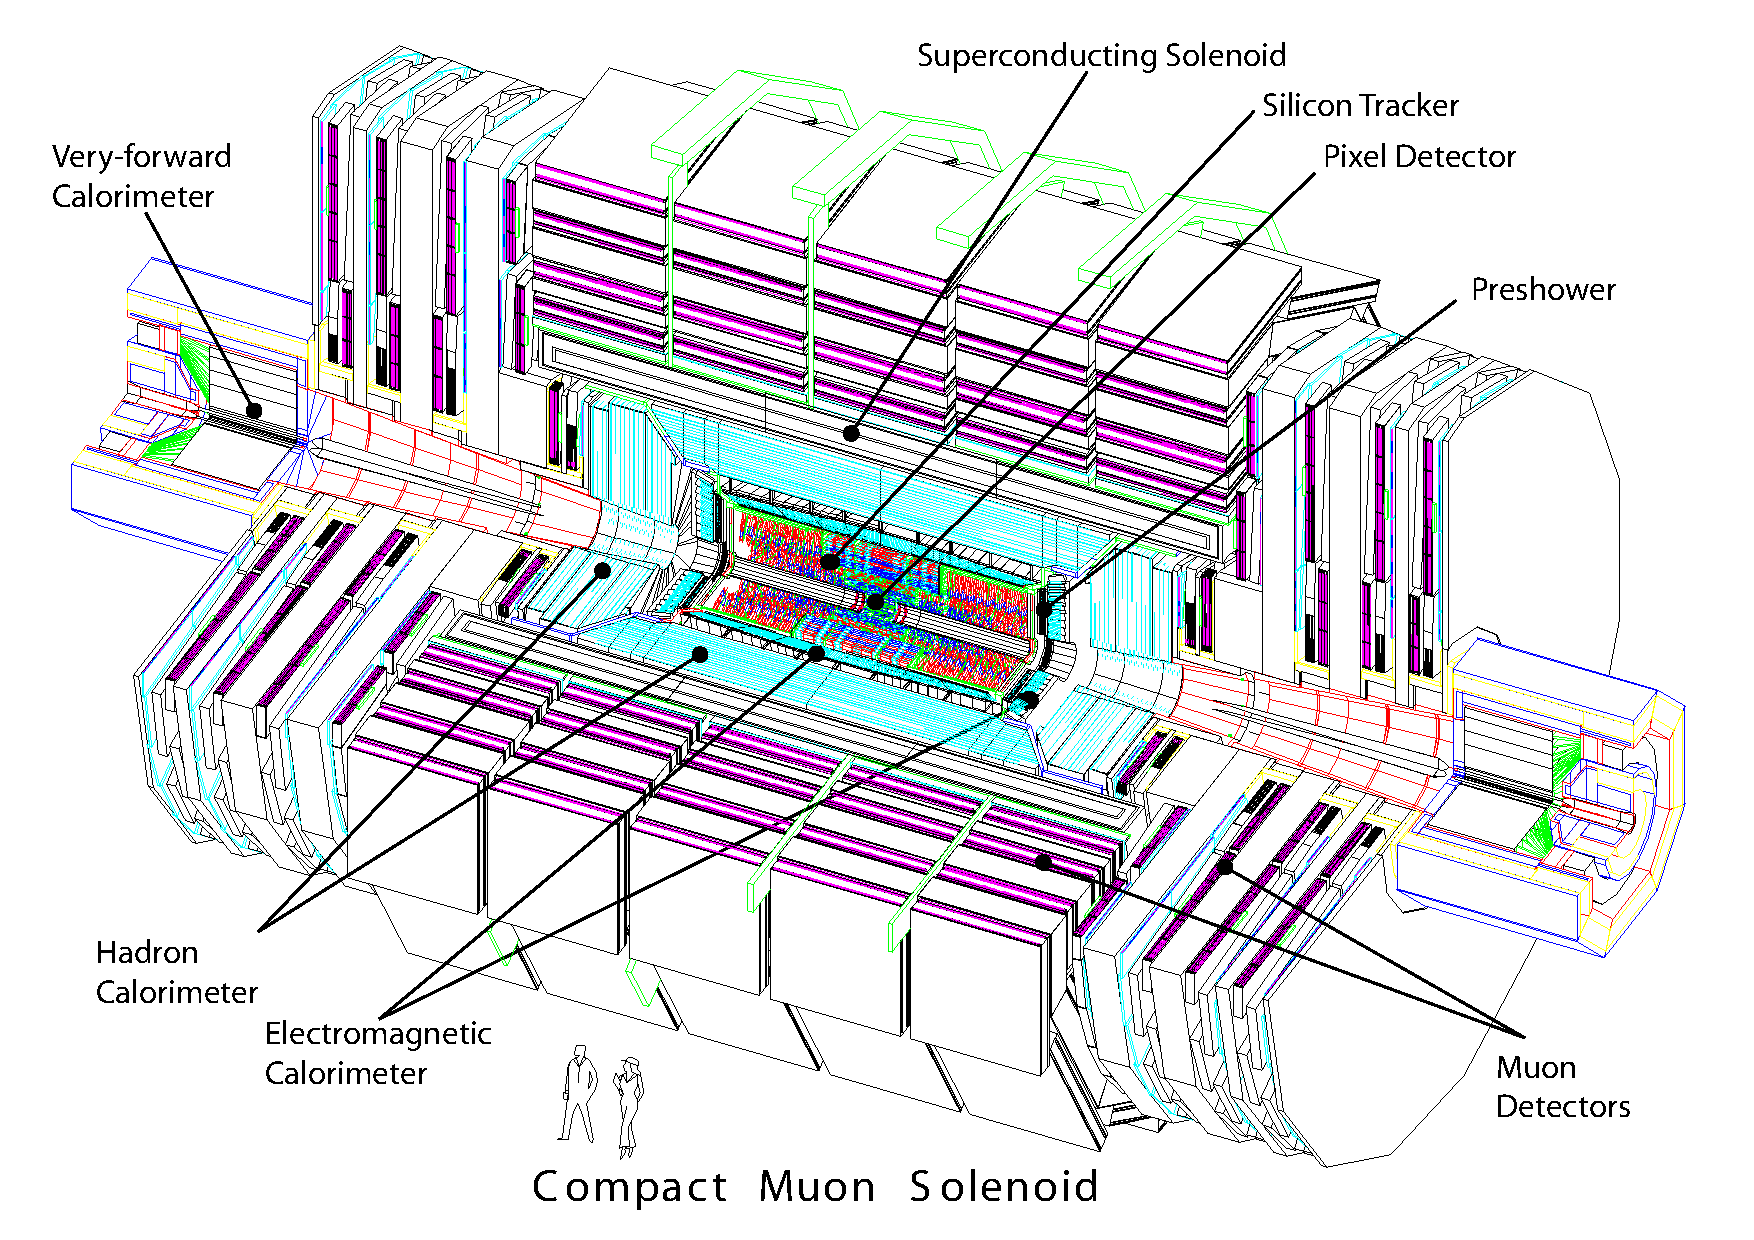
\includegraphics[width=0.9\textwidth]{Figures/Detector/CMS_Structure}
\caption[A cutaway diagram of the CMS detector structure identifying the main individual sub-systems.]{A cutaway diagram of the CMS detector structure identifying the main individual sub-systems~\cite{TDRVOLI}.}
\label{fig:CMS_Struct}
\end{figure}

The high magnetic field was chosen in order to achieve the bending power necessary for good charged particle momentum resolution. The inner bore of the solenoid is large enough that the inner tracker and the calorimeters are located inside, which minimises the material the particles pass through before entering the calorimeters. This improves the energy measurement resolution. Four muon ``stations" of aluminium drift tubes are integrated within the iron magnetic field return yoke. The full design description can be found in the CMS Technical Design Proposal \cite{CMSTDP}. As different particles pass through the detector they interact in the sub-systems depending on their type. A transverse slice through the detector illustrating the path through the machine of each type of particle is shown in Figure \ref{fig:CMS_Slice} 





\begin{sidewaysfigure}
\centering
\includegraphics[width=1.\textwidth]{Figures/Detector/CMS_Slice}
\caption[Transverse slice through the CMS Detector showing the path of each type of particle and how it interacts with the sub-detectors.]{Transverse slice through the CMS Detector showing the path of each type of particle and how it interacts with the sub-detectors~\cite{cmsslice}.}
\label{fig:CMS_Slice}
\end{sidewaysfigure}
\subsection{Coordinate System}

The coordinate system chosen by CMS uses the nominal interaction point within the detector as the origin. The x-axis points radially inwards to the centre of the collider ring, and the y-axis points vertically upward. The z-axis then points in the direction of the anti-clockwise beam. The azimuthal angle $\phi$ is defined as the angle from the x-axis in the x-y plane, and the polar angle $\theta$ from the z-axis. However, it is common convention to express $\theta$ in terms of the quantity pseudorapidity,~\begin{math}
\eta = -\ln \tan (\theta / 2) 
\end{math}, as particle production is approximately uniform in $\eta$. The transverse components of the energy and momentum, denoted $E_{T}$ and $p_{T}$ are then calculated from the $x$ and $y$ components. 



\subsection{Superconducting Magnet}

The geometry of the magnetic field is integral to the design and cylindrical structure of the CMS detector, as it uses a global solenoidal magnet. A strong magnetic field is essential to the design of a detector, bending charged particles in order to measure their charge and momentum. In order to ensure that the curvature is significant even with particles of high momentum, the CMS solenoid is designed to be capable of delivering a homogenous field of 4\,T within its volume. Consisting of four layers of NbTi coils in a vacuum with a cryogenic system maintaining a temperature of 4.5\,K, the solenoid has a diameter of 5.9\,m and length 12.5\,m, and when operating at full current is cable of storing 2.6~GJ of potential energy.

As the solenoid is so large, not only the inner tracking system but also both calorimeter sub-detectors can be accommodated in the interior, giving significant advantage to electromagnetic and jet energy resolution as particles will not have traversed the high-density magnet coil before these measurements are taken. The flux is returned with a large iron yoke of $10^{7}$~kg, surrounding the inner magnet and built with a barrel of 5 wheels, and two end-caps each containing three disks. The muon system is built within the iron return yoke, in order to take advantage of the reverse magnetic field produced in the outer region, and thus follows the same structure. The drawback of a solenoidal field is that it has strong inhomogenity in the end-caps, affecting the performance of the muon subsystem, which shall be discussed later.


\subsection{Tracker}



The first sub-detector encountered by particles is the multi-layer silicon tracker, which records precise information about the path of charged particles bending under the magnetic field. The inner layers are placed as close to the interaction point as possible in order to distinguish the primary interaction from secondary vertices of particles with significant lifetimes. This is particularly important in the case of identifying B mesons, which can travel a measurable distance before decaying.  

The tracker is divided into regions defined by the radius, $r$, from the interaction point, as the expected particle flux decreases rapidly as the radius increases. This is due not just to the increase in area of the solid angle, but also to the high magnetic field, which causes low momentum particles to have small radial helical trajectories.

Nearest to the primary vertex at 4\,cm, where the expected particle flux is at its highest ($\sim10^{8}$\,cm$^{-2}$\,s$^{-1}$), is the pixel detector which consists of 66 million silicon pixels of size 100 $\times$150\,\textmu m$^{2}$ arranged in three barrel layers and two end-cap disks. This region is laid out to optimise the resolution in determining the vertex position, delivering a hit resolution of $\sim$10\,\textmu m in the $r-\theta$ plane and $\sim$ 20\,\textmu m in the $r - z$ plane. Pixel detectors have the advantage of being able to measure all three coordinates of the particle simultaneously. However this requires a large number of readout channels and drives the costs of construction up. For this reason pixel detectors are chosen for the innermost region where the flux is highest, while the rest of the detector is composed of silicon micro-strip devices. 

Outside of the pixel detector lies the silicon strip tracker with its first layer located at $r$ = 20\,cm. It is divided into two parts, the inner and outer components. As the flux of particles expected is lower than in the pixel detector, the use of 11.4 million silicon strips allows the desired granularity while minimising costs. Whilst these do not allow a simultaneous 3-coordinate measurement, some of the layers are constructed at known angles to the others and therefore when combined all three coordinates can be measured. The inner region, immediately outside the pixel tracker, is composed of four barrel layers (TIB) and closed with three disks (TID) on each end, occupying the region up to $r$~=~55\,cm, where the microstrip sensors are 320\,\textmu m thick oriented along the beam line in TIB and radially in the TID. The outer region has 6 barrel layers (TOB) further apart than in the inner sector, and closed with 9 end-caps (TEC) on the end of the barrel, extending out to $r$~=\,116\,cm. The strips here are 500\,\textmu m thick.

In total the tracker covers a total area of 205\,m$^{2}$ with 76 million channels and provides a transverse momentum measurement for high momentum tracks with resolution 1 - 2\,\% in the region $|\eta| <$ 1.6.

\subsection{ECAL}

Immediately outside of the tracker, and still within the magnet core, sits the Electromagnetic Calorimeter (ECAL), used to measure the energy of electrons, photons and pions via the energy they lose through radiation. Electrons lose their energy in the material through \textit{bremsstrahlung}, and photons by decaying to an electron-positron pair. Using a hermetic homogenous calorimeter of scintillating crystals, this energy can be converted to scintillation light which is picked up by a light sensitive detector. 

The use of high density crystals allows a fast calorimeter which has fine granularity and is radiation resistant, requirements which are essential in the LHC environment. After rigorous research and development, lead tungstate (PbWO$_{4}$) crystals were chosen as the optimal solution to the requirements of LHC operation, due to a number of desirable characteristics. The extremely short radiation length $X_{0}$ = 0.89\,cm allows the construction of a compact ECAL which therefore can reside within the solenoid, hence reducing the amount of material particles have to pass through before reaching the calorimeter. In addition, the material has a small Moliere radius (2.2cm) meaning the transverse size of the electromagnetic shower is narrow, leading to good shower position resolution and separation. It is also essential that a fast scintillator is used, in order to distinguish between bunch crossings. In crystals of PbWO$_{4}$ 80\% of the scintillation light is emitted within 25\,ns, the bunch spacing of the LHC. Finally the crystals are hard to radiation, as their method of scintillation is resistant to radiation damage. 

The ECAL is structurally divided into three distinct regions, the End-caps (EE), the Barrel (EB) and the Pre-Shower (PS), which together cover a pseudorapidity range $|\eta| \leq$\,3. The ECAL Barrel is a cylindrical arrangement of 61200 PbWO$_{4}$ crystals covering the pseudorapidity range $|\eta| \leq$ 1.479 with a granularity of $\Delta \eta \times \Delta \phi = 0.0174 \times 0.0174$. The radius to the front-face of the crystals is 1.29 m. The crystals are wedge shaped with a front face surface area of 22\,$\times$ 22\,mm$^{2}$ and a back face area of 26\,$\times$ 26\,mm$^{2}$. The dimensions of the crystal are chosen to reflect the requirements, where the area of the front face is the Moliere radius squared and the longitudinal depth of the crystals is 230\,mm, which is 25.8 $X_{0}$ hence allowing a fine granularity and a compact ECAL. 


The ECAL is closed by two identical end-cap regions, which cover the range 1.479 $\leq |\eta| \leq$ 3 at the margins of the barrel, each consisting of 7324 crystals divided into two halves, or \textit{Dees}. Precision energy measurements are possible up to $|\eta|$ = 2.6, but crystals are included up to $|\eta|$ = 3 to assist the forward-direction energy-flow measurement. The end cap crystals are also wedge shaped with a square front face $28.62 \times 28.62$\,mm$^{2}$ and a square back face $30 \times 30$\,mm$^{2}$. The crystals point slightly away from the interaction point in order to make the end-caps hermetic, and are grouped mechanically into 5 $\times$ 5 super-crystals (SC). In the end-caps the presence of the PS allows for crystals of length 220\,mm, shorter than those of the barrel and corresponding to 24.7~$X_{0}$.

A additional component, the Pre-Shower is present in front of the end-caps covering a range of $1.653\leq |\eta|\leq2.6$ and consists of two layers of absorbing lead converters and silicon detectors. The primary function of the PS is to identify neutral pions that decay into two photons in the end-caps, which can fake high-energy photons. It also possesses a high granularity, and therefore is used to improve position determination of particles, and helps the identification of electrons against minimum ionising particles. The two layers of the PS have their strips orthogonal to one another such that the first layer has vertical strips and the second horizontal strips allowing better position resolution.

The crystals are read out using photodetectors, which convert the scintillating light of the crystals into an electric signal. The crystals were chosen by a rigorous optimisation of the properties required, which results in a high-performance ECAL, however this material has a relatively low light yield. In order to overcome this, photodetectors designed for use in a magnetic field with intrinsic gain are used. Vacuum Phototriodes  (VPTs) are used in the end-caps. These are unsuitable in the central region due to high magnetic field, but due to lower radiation levels Avalanche Photodiodes (APDs) are used. Both the crystals and the photodetectors are sensitive to temperature changes, so a stable temperature must be maintained. Radiation damage to the crystals decreases with temperature, but so do the thermal effects which result in recovery. The operational temperature, 18\,\textdegree C is chosen as it is the point of equilibrium between damage and recovery.


The resolution of an ECAL can be described as a function of the energy, $E$, in GeV, shown in Equation \ref{eq:E-Res}, for energies below about 500 GeV~\cite{PDG}. Above this shower leakage from the back of the crystals becomes non-negligible. 
\begin{equation}
\left(\frac{\sigma}{E}\right)^2 = \left(\frac{S}{\sqrt{E}}\right)^2 + \left(\frac{N}{E}\right)^2 + C^2
\label{eq:E-Res}
\end{equation}
The stochastic term, $S$, represents fluctuations related to statistics, including photoelectron statistics and intrinsic shower variations. The noise term, $N$, takes into account electronic noise summed over readout channels, and the constant term, $C$, accounts for the uncertainty in calibration and the detector non-uniformity. Measurements from test beam reconstructed energy distributions show values for the terms to be $S$\,=\,2.8\,$\pm$\,0.1\,\%, $N$\,=\,0.12\,GeV and $C$\,=\,0.30\,$\pm$\,0.01\,\%. 


\subsection{HCAL}

Outside the ECAL lies the Hadronic Calorimeter (HCAL),  responsible for the measurement of the hadronic activity of an event. This also leads to a measurement of apparent missing energy from neutrinos or exotic particles, an important quantity in many searches for new physics. In order to measure the energy of hadrons in a compact space, a sampling calorimeter of interleaved layers of absorbers and scintillators is used. The absorbing material forces hadronic showering through nuclear interaction with heavy nuclei, and the active scintillating material then samples the showers of charged particles produced. The absorber material is described by the interaction length $\lambda_{I}$, the distance a hadron will travel through the material before it has lost roughly 63\% of its energy through nuclear interactions.

 The HCAL is divided into several sections, defined by pseudo-rapidity in order to optimise the resolution under different conditions. Within the space between the ECAL and the magnet coil lie the HCAL Barrel (HB) at $|\eta| < 1.305$, and the HCAL End-Caps (HE) at $1.305 < |\eta| < 3.0$, hermetically joined to completely surround the ECAL. In order to increase the hermicity of the HCAL, and therefore improve the accuracy of the missing energy measurement, the two elements of the HCAL Forward calorimeter (HF) overlap with the HE and extend the range in pseudorapidity to $|\eta|<5$. There is also a complimentary layer of scintillators on the outside of the coil, known at the HCAL Outer (HO).  This provides shower containment in the central region, where the number of interaction lengths travelled by a particle is at its lowest~\cite{HCALTDR}.


\begin{figure}
\centering
\includegraphics[width=0.8\textwidth]{Figures/Detector/HCAL}
\caption{Diagram of one quadrant in the r-$\theta$ plane showing the locations of the components of the HCAL: HB, HE, HO and HF, with lines of constant $\eta$ shown.}
\label{fig:HCAL}
\end{figure}


The barrel consists of two halves each with 18 identical azimuthal wedges, extending outwards by 0.96\,m. Each wedge has 17 layers of 3.7\,mm thick plastic scintillator, interspersed with brass absorber plates, with the exception of the innermost and outermost absorbers, which are made from stainless steel to add structural stability. Directly behind the ECAL is placed the first active layer, with more than double the scintillator thickness (9\,mm) to actively sample the particles traversing the support material between the ECAL and HCAL. The final layer also has this thickness to catch showers that form late in the absorber. 

A similar structure makes up each end-cap with 18 wedges dividing up the angle $\phi$ containing 19 active plastic scintillators with brass absorbers between. The number of interaction lengths travelled by particles in the HB and HE is dependent on the $\eta$ of the particle, and while it is 10 at high $\eta$, in the central region this is as low as 5. In order to compensate for this, an outer barrel detector is added in the range $|\eta| <$ 1.26 consisting of two layers of scintillating material outside the magnet, and therefore utilising the coil as an absorber. This extends the total thickness of the full calorimeter to at least 11.8 interaction lengths. 

The design of the forward calorimeters is driven by the need for radiation hardness, as the region closest to the beam line has an energy density up to seven times greater than in the central region. Thus absorbers made of stainless steel and active scintillators of quartz fibres are chosen. Twelve wedges in $\phi$ are located 11.2m from the point of interaction, with the fibres parallel to the beam.

Measurements of hadron energies in the region $| \eta| < 3.0$ rely not only on the HCAL setup described, as a significant fraction of hadrons will have begun to shower while travelling through the ECAL, which contributes around one interaction length.  The hadronic component of these showers will continue on into the HCAL, but much of the initial electromagnetic activity can be contained in the ECAL, thus use of measurements in both calorimeters are combined to reconstruct the true energy of a hadron. Using test beams over a range from 2 to 350 GeV the resolution for the reconstruction of hadron energy for the HCAL and ECAL combined is given by the following equation~\cite{HCALTestBeam}.
\begin{equation} 
\left(\frac{\sigma}{E}\right)^2 = \left(\frac{84.7\%}{\sqrt{E}}\right)^2 + \left(7.4\% \right)^2 
\label{eq:H-Res}
\end{equation}


\subsection{Muon System}

Interleaved in the iron return yoke of the detector are the components of the Muon System (MS), an important design feature giving CMS its middle initial. Many new physics signatures at high energy have final states with high momentum muons, and therefore accurately measuring these is crucial for many analyses, including Higgs and SUSY channels. As muons are high mass leptons they interact little in the calorimeters, and thus retain a high percentage of their energy by the time they reach the iron return yoke. Putting the MS here far away from the interaction point allows finer precision, utilising the high magnetic field to bend even high momentum muons, and measuring the bending angle. This allows a finer precision for muons with  $p^{\mu}_{T} > $ 200 GeV.

%Muon momentum resolution using the MS is constrained at low energies (0 $< p^{\mu}_{T} < $ 200 GeV) by both the multiple scattering that occurs in the material prior to the first muon station, and therefore a better resolution could be obtained using the tracking system. However, it is possible to use the muon trajectory after the yoke to extrapolate back to the interaction point. 

Low momentum muons (0 $< p^{\mu}_{T} < $ 200 GeV) are measured more accurately in the tracker than in the MS as they undergo multiple scattering in the material budget prior to the MS. However, using the tracker and muon system together improves identification and measurements, especially as any particle detected in the MS is expected to be a muon, as other particles are stopped earlier in the detector~\cite{MuonTDR}. Muon reconstruction is discussed in further detail in Section~\ref{sec:muona}. 

Built within the iron yoke the MS shares the same structural layout, constructed in five barrel wheels, and two end-caps, together covering the region $|\eta| < 2.4$. As a large area must be covered, a silicon based setup such as used in the inner tracker would be too expensive, hence gaseous detectors are chosen. In the barrel region ($|\eta| < 1.2$) Drift Tubes (DT) are used, and in the end-caps ($0.9 < |\eta| < 2.4$) Cathode Strip Chambers (CSC) are preferred, both of which offer good position resolution, although they have a long response time. In order to provide redundancy in the trigger system an additional third element is added in both regions, the Resistive Plate Chambers (RPC). These have a worse position resolution but benefit from a much shorter response time suited to identifying the bunch crossing. Combining the information from these complimentary RPCs with the DTs and CSCs gives rise to an efficient and robust trigger. The arrangement of the muon system is shown in Figure~\ref{fig:MuonSystem}, with the locations of each type of detector shown.

\begin{figure}
\centering
\includegraphics[width=0.6\textwidth]{Figures/Detector/MS}
\caption{The Muon system shown in the $r-\theta$ plane showing the three components and their locations. Lines of constant $\eta$ are indicated for reference.}
\label{fig:MuonSystem}
\end{figure}

In the barrel, the magnetic field is uniform, and therefore allows the use of Drift Tube chambers.  Each of the five wheels are made up of 12 sectors, containing four chambers apiece, making up a full barrel of 240 chambers. The inner three chambers consist of three Super Layers (SL) using the first and third for the $\phi$ coordinate measurement and the second for the $z$ coordinate. In the outer chamber,  there are only two SLs and these contribute only to the $\phi$ measurement. Four layers of drift tubes make up a SL, and each layer is shifted by half a cell from the one beneath, to ensure any particle trajectory meets some active material. Each tube contains an anode wire and cathode strips, and is filled with a gas mixture of 85\% Ar and 15\% CO$_{2}$ gas. The Ar atoms are ionised by a charged particle, and the resulting electrons and ions drift towards the anode and cathodes. Electrons reaching the wire are extremely excited by the high density field, which allows them to ionise further molecules, known as the ``avalanche effect". Thus an electrical signal large enough to be measured is produced. The drift distance is 21\,mm and the drift time is limited to $\sim$\,380\,ns by the gas chosen, corresponding to 16 bunch crossings.

Due to the aforementioned solenoidal magnetic field, the end-caps experience an irregular magnetic field, and a higher expected particle flux, and therefore drift tubes are not suitable. In this region 468 Cathode Strip Chambers are used, set out perpendicularly in four stations in each end-cap. Trapezoidal chambers consist of seven radially oriented cathode strips, and in between six planes of azimuthal anode wires. The gas filling the gaps is made up of 40\% Ar, 50\% CO$_{2}$ and 10\% CF$_{4}$, and the chambers work much in the same way as the DT's, with a high voltage applied to achieve the avalanche effect. As the wires and strips are almost perpendicular its possible to make a simultaneous measurement in r and $\phi$ by identifying the charge fraction in several cathode strips. 

In addition, the complimentary system of RPCs is installed in both the barrel and end-cap regions, providing extra information in the region $|\eta| < 1.6$. In the barrel there are 480 rectangular RPCs, with two layers per station, the inner two stations have one inside and one outside the DTs, and the outer two stations having both inside. The end-caps have overlapping trapezoidal chambers in the outer two concentric rings. These parallel-plate gaseous detectors have two thin gaps between plates, which are attached to high voltage to drive avalanche mode. The avalanche reaches the plates quickly, as the gas gaps have a small width, and so the measurement is made within $\sim$\,3\,ns, much smaller than the bunch crossing. The position resolution is adequate at the same time, and so the RPCs are used to contribute to the trigger, and also to map identified muons to a particular bunch crossing.

\subsection{Trigger}
\label{sec:detrig}
When running at design luminosity, the LHC will collide protons with a bunch crossing of 25~ns, each of which will result in $\sim$\,20 interactions corresponding to a rate of 40MHz of data, or 40\,TB/s~\cite{TRIGTDR}. Not only is it impracticable for this volume of data to be stored, but much of this corresponds to unwanted events, where no new particles have been produced, as the cross-sections for interesting physics processes are several orders of magnitude lower than the inelastic p-p cross section. Hence these events must be whittled down into those which it is worthwhile to store. This is done by the trigger system that is divided into two components, the online hardware-based Level 1 Trigger (L1) which reduces the rate to that which can be routed from the buffer to the computing farm, and then the offline software-based High Level Trigger (HLT). 

The L1 trigger is driven by the amount of time that data at the incoming rate that can be stored in the buffer, before needing to be overwritten. At design luminosity this is 128 bunch crossings, $\sim$\,3\,\textmu s. Within this time the rate must be lowered to 100kHz, the acceptable rate for writing to the computing farm used for the HLT. This is accomplished using a tree system of triggers. First, the Regional Calorimeter Trigger (RCT) and Regional Muon Trigger (RMT) perform local reconstruction of objects (muons, electrons, photons, jets). The Global Calorimeter Trigger (GCT) and the Global Muon Trigger (GMT) receive these objects, and sort them using a number of criteria e.g. Energy, momentum, quality of identification. The top four of each type are sent to the Global Trigger, which uses this information along with global event measurements such as total momentum to decide if the event passes the L1 Trigger requirement. If so it is sent to the HLT, if not it is not stored and passes out of the buffer. 

The HLT essentially does the same thing as the L1 trigger, but is not driven by strict time requirements. Running on a large computer farm of multi-core computers, it has access to the entire readout data, and performs sophisticated calculations akin to those performed in physics analyses. Using partial reconstruction algorithms to clearly identify what objects are in an event, it is possible to filter according to a set of desired physics criteria.  The desired rate to store to tape is around 300Hz, and the HLT is designed and monitored constantly during data-taking to ensure the correct rate is achieved. In a given run a ``menu" of different trigger paths is included, to select different types of event and with different thresholds. Some require the presence of a certain object, such as a Muon. Others combine requirements, and these are called Cross-Triggers. For example a family of triggers exist that require a certain HT and MHT. Within this family there are several different thresholds, which go down as low as can be included in the menu without raising the rate prohibitively much. Thresholds that have a rate which is too high become ``prescaled".
\subsubsection{Prescaled Triggers}
If the rate of output of a given trigger becomes too high as the luminosity increases, the trigger will often remain in the menu with a lowered rate due to the inclusion of a ``prescale factor" $n$. The trigger is known as ``prescaled", as only 1 in $n$ events that pass the trigger requirements will be included in the trigger output, thus reducing the efficiency of said trigger by the factor $n$. 

For analysis search purposes this is undesirable as it would result in a significant loss of interesting events, but these prescaled triggers can play a part in control samples and background estimates. In these areas it is suitable to multiply the yield by the prescale factor in order to provide an estimate of actual event numbers, whereas in the signal region it is essential to treat only physical yield measurements with an un-prescaled trigger.
\subsection{Primary Dataset}
Several Primary Datasets (PD) are used to store the data, where an event is allocated to a PD based on which low-threshold trigger bits are passed in order to group like events together. For example, in this thesis the datasets used are the HT PD where events are stored that pass low requirements of missing energy, and also the Photon PD in which events have at least one photon. This is done for ease of use of the analysis user. The PDs have some overlap, therefore only one is required for a full luminosity analysis providing the offline selection is efficient to the triggers used in selection. In the analysis set out in this thesis the use of the Muon PD is rejected for the muon control sample for this reason, as the selection allows very soft muons. 



\chapter{Event Reconstruction}

The data stored directly from the CMS detector readout contains only the most basic level of information of a collision. As the particles created in the event pass through the detector they create signals at each point they interact, and these signals are locally reconstructed a s a series of ``hits". This raw data is stored in CMS as the data format RAW. In order to undertake physics analyses the information is needed in terms of the four-vectors of particles. In order to interpret the raw data in terms of these physics objects a computational process known as object reconstruction is applied to the data. Using knowledge of the behaviour of each type of object and understanding of the detector, the objects are built from the hits, in such a way that optimises the efficiency for each type of object. Varying sets of requirements called ``identification" or ID can then be applied to these objects at the analyses level to achieve the level of purity required. 

The reconstruction of physics objects happens both within a sub-detector, and also by combining information from two or more sub detectors. The reconstruction is performed under the CMS Software framework (CMSSW) and the reconstructed data is stored in RECO format for use by individual analyses. The analysis in this thesis requires the use of jets, \met, muons,  and photons, with electrons required for a veto.  

\section{Tracks}

Whilst not a physics object in its own right, one of the most important elements of object reconstructions involves the identification of tracks left by charged particles in the inner tracker. There can then be used along with other sub detectors when reconstructing charged physics objects. In addition these tracks allow a precision identification of the vertex of interaction. In CMS an algorithm called the Combinatoral Track Finder (CTF) is used to construct tracks from their representative hits. 

The reconstruction of a track starts with the construction of a ``seed", an initial candidate track. It contains only a small subset of the available information from the tracker, but must be made up of at least 3 hits, or two hits and an additional beam constraint. The seed represents the initial estimate of the track's trajectory, from which to collect its additional hits. In order to achieve the best possible estimate, the seed is built from hits in the innermost area of the tracker, for three important reasons. Although in general the average occupancy decreases with r, the high-density nature of the pixel detector ensures the inner layer of pixel detectors has an occupancy lower than that of the outermost strip detectors. In addition, the pixel detectors give a better estimate of the trajectory due to their truly 2D measurements, and constructing them in the innermost layer minimises the material budget encountered, as not all particles will reach the outer layers. 

The next element of CTF is a patter recognition module based on a Kalman Filter, that proceeds from the seed outwards and includes any additional hits associated with the basic estimated trajectory. As each new measurement is incorporated to the track the trajectory becomes more accurate. This proceeds for each track candidate in parallel, and where several hits are compatible several new candidates are created. In order to safeguard against reconstructing one particle as more than one track, an ambiguity resolution mechanism is needed Given any pair of track-candidates, the fraction of shared hits in the candidate with the fewest hits is examined, and if found to be greater than 50$\%$ this track is removed. If the number of hits is identical then that of the lower $\chi^{2}$ remains while the other is removed. 


Once all compatible hits have been incorporated the tack parameters can be extracted using 




\section{Vertex}
\section{Electrons}

\section{Muon}
\section{Jet}

\chapter{Searching for SUSY with $\alpha_{T}$}
\label{ch:at}

The data collected by the CMS detector could hold signs of physics Beyond the Standard Model (BSM). In order to search for signs of new physics they must be distinguished from the vast quantity of Standard Model processes that will arise. Due to the nature of hadron collisions, a large background from QCD events is present, which poses challenges unlike the clean lepton colliders. The events one wishes to look for are termed ``signal" events, and all others become part of the ``background". Search strategies are developed to optimise the selection of desired events whilst rejecting a large proportion of the unwanted ``background" events. The validity of a search is tested using Monte Carlo simulations of both possible signal and expected background events, and is often evaluated by the proportion of signal S to background B, the S/B of a search. 

This thesis focuses on searching for new physics inspired by almost all SUSY models. In this chapter we explore the nature of such new physics and the development of a new variable \alt which forms the backbone of a search for events with quarks and a large quantity of missing energy. 

\section{Inclusive SUSY Search}

As previously discussed in Chapter \ref{ch:theory}, SUSY models that conserve R-Parity and therefore indicate new physics at the TeV scale introduce a candidate particle for dark matter. As this LSP cannot be observed due to its weakly interacting nature, searching for it is analogous to a search for large missing energy in particle collisions. In the CMS detector reconstruction of all visible particles allows us to calculate the transverse component of this quantity, missing $E_{T}$ or \met. 

As there are many models to describe the exact nature of SUSY due to the unknown mechanism of SUSY breaking, it is desirable to design an experimental search which does not rely on any one in particular, or even on the assumption of SUSY. These are called ``inclusive" searches, and retain sensitivity to any new physics resulting in a new particle with the properties of a WIMP. The main feature is a requirement of a large quantity of \met along with final state objects (hadronic jets, leptons, photons). The search space is then divided into channels via the final state objects required, in order to perform orthogonal searches to increase sensitivity and to allow combination 

Discussion of SUSY on the whole and specific models such as mSUGRA are then used to quantify the reach of the search and to tune the cuts with Monte Carlo data. Where no new physics is found it can be useful to set limits on the parameters of such models, and in this thesis we will use mSUGRA for this purpose, along with test points in the mSUGRA phase space. However it is important to remember that the search itself remains open and sensitive to any WIMP candidate. 

Physics at the LHC will suffer from high background rates, especially those from QCD, and the main goal of any analysis is selecting the new physics events required whilst removing the background from Standard Model processes. Missing energy can be observed in events in two ways, real missing energy from the production of weakly interacting particles, such as neutrinos and LSP's, and fake missing energy which is a result of mismeasurment of objects, or missed objects. 

Having noted that the generic signal produced by any such new physics model is a large amount of \met, it might be assumed this forms the main variable to separate signal from background events. As \met is measured in the calorimeters, it can be affected by miscalibration and noise in the detector, thus is not robust for early physics at the LHC. 

To combat this issue there is also the quantity \mht which represents the vector sum of transverse momenta $p_{T}$ of the jets in the system, giving the hadronic missing energy analogous to \met in a hadronic search. However, there are limitations to the use of either of these quantities, as they are not robust to mismeasurments of the jets. 

A background event with no missing energy may therefore be selected as having considerable \met or \mht due to these mismeasurments, and thus it is natural to look for other variables which have a higher discriminatory power. 







\section{$\alpha_{T}$ in a di-jet system}

The first step in devising a SUSY search strategy begins with the simplest of channels, the ``dijet" search with just two jets and missing energy corresponding to two missing neutralinos.  This channel is motivated by one of the cinematic scenarios of mSUGRA mentioned in Chapter \ref{ch:theory}, where the gluino is heavier than the squarks, therefore squarks are liable to decay directly to the LSP producing a quark jet. Due to the low multiplicity it is easy to understand kinematically the situation in play. 

At the LHC the dominant background is from QCD diet events, produced with an extremely large cross section. These events do not actually produce \met but can ``fake" this signature through detector effects such as mismeasurment or missed objects. In addition there are a number of other backgrounds that produce real missing energy in electroweak interactions, W + jets, $t \bar{t}$ and Z $\rightarrow \nu \bar{\nu}$ + jets, which we will refer to collectively as EWK. The greatest task on hand is to eliminate the dominating QCD background, which in a perfect detector could be easily achieved with a simple cut on \met or \mht. However, due to the ``fake" \met signature from QCD events, a significant proportion of these events remain after such a cut, so it is desirable to devise a variable which can separate true sources of missing energy, and those arising from the detector. 

In a QCD diet event, were it to be perfectly measured, the two jets are pair produced and following conservation laws must be back-to-back and of equal magnitude. In events with real missing energy, such as our potential SUSY signal, the jets have been produced independently of one another, and such rules do not govern them. The distribution of the azimuthal angle between the two jets, $\Delta \phi$, is therefore very different for the QCD background and potential signal events.  


It is possible to exploit the nature of this further using a new variable proposed by Randall and Tucker-Smith, $\alpha$, defined in Equation \ref{eqn:alpha}~\cite{Randall}. 

\begin{equation}
\alpha = \frac{E_{T}^{j2}}{M_{inv}^{j1,j2}}
\label{eqn:alpha}
\end{equation}

The $E_{T}^{j2}$ is the transverse energy of the second jet (the lowest in energy) and $M_{inv}^{j1,j2}$ is the invariant mass of the dijet system. The design of this variable allows us to exploit the expected back-to-back nature of any dijet from QCD. A well-measured QCD event can only take values of $\alpha < 0.5$. In sharp contrast, a SUSY event can, due to the unseen neutralinos, produce jets in a similar direction with a low invariant mass giving rise to high values of $\alpha$.

The transverse variant of this variable, given in Equation \ref{eqn:alpha} makes use of the transverse mass $M_{T}$ of the two jets as opposed to the invariant mass.

\begin{equation}
\alpha_{T} = \frac{E_{T}^{j2}}{M_{T}} 
\label{eqn:alphat}
\end{equation}

In this case a well-measured QCD event will have exactly 0.5. While both show equally strong power of background discrimination, $\alpha_{T}$ has greater signal retention for certain mSUGRA points,\cite{PASaT} and therefore is deemed comparable or superior. It is upon this variable that the search strategy is formed. The presence of the second jet energy in the numerator also gives rise to one of the most important properties of this variable, its resilience to jet mismeasurment. If there is a large mismeasurment of one of the jets, the order could be inverted. As a perfectly measured QCD event yields \alt = 0.5, the cut chosen is \alt > 0.55 in order to take into account the finite resolution of the jet energy measurement.  


The explicit reliance of \alt on $\Delta \phi$ can be seen when the relationship is rewritten in the massless limit, in Equation \ref{eqn:alphatphi}. This relationship indicates a high correlation, and thus a cut on \alt renders a further cut on $\Delta \phi$ negligible\cite{ANaT}.

\begin{equation}
\alpha_{T} = \frac{\sqrt{E_{T}^{j2}/E_{T}^{j1}}}{2(1- \textrm{cos} \Delta \phi)} 
\label{eqn:alphatphi}
\end{equation}


\section{$\alpha_{T}$ in a n-jet system}
More complicated decay processes result in hadronic signatures with more than two jets, generalised to the n-jet system, for example where a gluino-squark pair decay to produce three quarks and two LSP's. In order to increase phase space the dijet search channel may be extended to a final state including N jets and considerable \met, where N $\geq$ 2. This is colloquially known as the all-hadronic search channel as it comprises any fully-hadronic decay modes that might yield possible SUSY signal. 

Following the success of the construction of the \alt variable in the dijet topology, the variable was extended to a general form applicable for an n-jet system, thus incorporating the full hadronic SUSY search channel\cite{ANnaT} . This is undertaken by modelling the system of $n$ jets as though it were a diet system, through the mathematical construction of two pseudo jets. Thus \alt can be calculated using the properties of the pseudo jets. 

The two pseudo-jets are built by merging the n jets present in two sets with a vectorial sum deciding the direction, and a length equal to the sum of the magnitudes of the composite jets. The combinations chosen to assign n jets into 2 pseudo jets is done such that they are as balanced as possible, i.e. the difference in \HT, $\Delta \HT$ is at a minimum. All combinations are therefore considered, and the one which satisfies this condition is chosen. With this psedo-dijet system we can construct a formalism for \alt that uses the basic kinematic variables of the system in Equation \ref{eqn:alphat_njet}. 

\begin{equation}
\alpha_{T} =\frac{1}{2} \frac{(\HT - \Delta \HT)}{\sqrt{\HT^{2} - |\mht|^{2}}}  = \frac{1}{2} \frac{1-\Delta \HT / \HT}{\sqrt{1 - (\mht / \HT)^{2}}}
\label{eqn:alphat_njet}
\end{equation}

The second form of the definition shows its dependence on the ratios of $\Delta \HT$ and \mht to the events \HT. In a well measured QCD event there is no \mht, and $\Delta \HT / \HT < \sfrac{1}{3}$, from which the maximal value comes from the rare ``Mercedes Star" QCD event with three jets of equal mass and momenta with the $\Delta \phi$ between any chosen two being equal. Therefore with an ideal detector QCD events have $0.333 < \alt < 0.5$, but large mis-measurment leads to a high \mht which can higher the values of \alt. The chosen cut value of \alt $>$ 0.55 corresponds to a missing energy fraction \mht / \HT $>$ 0.4, and as this occurs in QCD events the ratio $\Delta \HT / \HT$ is liable to increase also. This relationship prevents \alt for QCD events from significantly exceeding 0.5 unless an object of sizeable momentum were missed altogether in the calculation. 

It has been shown that whilst the sharp cut-off for QCD events at \alt = 0.5 becomes less distinct, it is still pronounced as can be seen in Figure~\ref{fig:atedge} and thus retains the powerful background rejection properties desired\cite{an2009_56}. Performance tests with smeared jet energies shows the \alt variable applied to a multi-jet analysis is robust to jet mis-measurment, and superior in this area to a standard \met analysis. The jet energy scale does not directly affect \alt but its resolution improves for increasing \HT, as demonstrated with 7 TeV data in Reference \cite{an2010_119}. 

\begin{figure}[htbp]
\begin{center}
\includegraphics[width=0.6\textwidth]{Figures/AlphaT/ThesisATPlot}
\caption{\label{fig:atedge}Distributions of \alt in multi-jet events form Monte Carlo for QCD and the electroweak backgrounds W, \tto and Z + jets, indicating the sharp edge around the standard cut value of 0.55. Also shown are the distributions of the two SUSY CMSSM test points LM4 and LM6.}
\end{center}
\end{figure}


\section{Defining the ratio \RaT}
\label{sec:atrat}

The proportion of SUSY signal to background differs greatly with the \HT of the event, with background processes dominating at low values while SUSY becomes more prominent for high \HT. In order to investigate this behaviour a new variable \RaT is defined in Equation \ref{eqn:rat} as the ratio of events passing the cut \alt $> X$ with those that fail it, where X is normally 0.55. 

\begin{equation}
\RaT(X) = \frac{N(\alt > X)}{N(\alt < X)}
\label{eqn:rat}
\end{equation}

The relationship of this variable with \HT that can then be studied for background processes and potential SUSY signal using Monte Carlo samples. Where QCD events with no real missing energy dominate the numerator, tightening the \HT cut results in a decreasing \RaT. If the QCD background is negligible due to a successful \alt cut, the now-dominating  electroweak backgrounds contribute some real missing energy in the form of neutrinos and exhibit a flat relationship with \HT. However, in the presence of an mSUGRA SUSY signal in the numerator an increase of \HT corresponds to an increasing \RaT. These three distinctive behaviours provide a strong search strategy using \RaT in exclusive bins of \HT. These trends have been shown to be robust to jet mismeasurments, or even when 1 jet in 25 is not included in the calculation \cite{an2010_119}



\section{Extending $\alt$ for single-lepton searches}
\label{sec:lalt}
A cleaner SUSY signature can be obtained through the single lepton channel, where the topology identical save the extra requirement that there be one muon or electron in the final state. In addition, requiring a lepton can provide a useful control sample for the hadronic search. Hence it is interesting to develop the \alt search to apply to this channel, especially where the lepton $p_{T}$ is low and hence the dominant background is from fake leptons in QCD events. 

In this case, in the final state there is one lepton, and n jets where n is at least two. Production mechanisms for one lepton and two jets in SUSY decay modes at the LHC are similar to those of the 3-jet hadronic channel. Thus it is possible to draw parallels, and describe the system as an n-object system. Here, an n-jet hadronic event is treated the same as that which has 1 lepton and n-1 jets.  The quantities in the definition of \alt are extended to include the lepton as if it were a jet, such that the lepton is included in the building of the two pseudo-jets. 

The validity of this approach can be seen in Figure \ref{fig:aTnobj} where the hadronic (0-lepton) and single leptonic (1-lepton) cases are shown superimposed for the SUSY test point LM0, for three different object multiplicities 3, 4 and 5\cite{an2009_188}. As can be seen, although the shape of the \alt distributions change with the object multiplicity, there is a good agreement between the n jet system and the n-1 jet plus lepton system. 

\begin{figure}
\centering
\includegraphics[width=0.45\textwidth, angle=90]{Figures/AlphaT/aT_3}
\includegraphics[width=0.45\textwidth,angle=90]{Figures/AlphaT/aT_4}
\includegraphics[width=0.45\textwidth,angle=90]{Figures/AlphaT/aT_5}
\caption{\label{fig:aTnobj}The shape of the \alt distributions for object multiplicity N for the N-jet channel (0-lepton) and the N-1 jet plus 1 lepton channel superimposed. From left to right the object multiplicities shown are N=3, N=4, N=5.}
\end{figure}

\section{Reliance of \alt on jet object definition}

As mentioned above, although \alt is robust to mismeasurments a large value can be obtained from a QCD event if significant objects are not included in the measurement. To remain within the capabilities of the detector and reconstruction algorithms, the definition of a jet for the purpose of analysis requires the passing of a certain jet energy threshold. As this value is relatively small compared to the total \HT of an event, it should not contribute a large mismeasurment effect to the \alt variable. However there might be some cases for high jet multiplicities where a large number of low-energy jets just below the threshold are not considered, and so the \alt value is skewed. Hence, to remove this effect it is possible to make a cut in the ratio of the missing energy estimated from jets \mht and that measured by the calorimeter systems \met so that an event with $R_{miss} > 1.25$ is rejected. 

\chapter{The all-hadronic search with inclusive jets + missing energy}
\section{Event Selection}
\section{Analysis and Results}
\section{Data-Driven Background Estimation}
\subsection{Total background prediction}
\subsection{Estimating EWK background using high $p_{T}$ using W+Jets events}
\subsection{Estimation Z  $\nu \bar{\nu}$ + jets background using photon + jets events}
\section{Systematic Uncertainties}
\section{Limits}
\section{Conclusion}


%\chapter{Extending the Muon Control Sample to a Signal Sample}
\label{ch:ra4}

In Chapter~\ref{ch:ra1}, the muon control sample was used to predict the background contribution from W and \tto events. The muon likelihood's incorporation into the total likelihood in order to interpret the hadronic results allowed for some small signal contamination. However it was, in general, viewed as a constraint on the ``signal" region of the hadronic selection. 

The selection outlined in Section~\ref{sec:muon} was designed to select events from Standard Model W decays, hence minimising the contamination from signal. However, as the simultaneous fit includes the signal efficiency in the $\mu$ control sample it is possible to relax the cuts and allow more potential signal into the $\mu$ yield. Instead of viewing it as a control sample it may then be considered as a second signal sample in the simultaneous fit. The electroweak background behaviour is still constrained by the flat behaviour in \RaT whereas the presence of signal would exhibit an exponentially increasing behaviour. Thus it is possible to construct a dual-sample search in order to extend the reach of the analysis.  The following work represents the author's personal investigation into the effect of increasing the chance for signal contamination in the $\mu$ selection on the eventual limit with the current dataset. 

\subsection{Relaxing the Cuts}

The primary cut in the $\mu$ control sample responsible for restricting the signal is the $M_{T}$ requirement, as it puts a restriction on boosted W decays. The first step is to remove this cut, allowing more potential signal into the sample. Having done so there are three possible scenarios with respect to the \alt cut. Using the \alt cut as defined in the hadronic analysis is a natural choice. However the use of an \alt cut limits the statistics, so removing this cut would increase the muons sample statistics. Conversely, using the hadronic definition of the \alt cut where the muon is not considered leads to the false appearance of missing energy, hence allowing more background into the sample. The use of the leptonic version of \alt, $\alpha^{lep}_{T}$ in the cut as defined in Section~\ref{sec:lalt} does not suffer from this issue, but as this is a tighter cut will reduce the available statistics. 

The four $\mu$ selection criteria considered are therefore:

\begin{itemize}
\item 2011 Selection (unchanged)
\item a) No $M_{T}$ Cut and use the \alt $> 0.55$ cut from the hadronic analysis where the muon is ignored (as previously in the 2011 selection)
\item b) No $M_{T}$ Cut and take out the \alt cut (the $\sfrac{\MHT}{\HT} >$ 0.4 cut ensures the elimination of QCD background is maintained)
\item c) No $M_{T}$ Cut and make a cut with the leptonic \alt, $\alpha^{lep}_{T}$ $>$ 0.55
\end{itemize}

The one muon requirement cut and the other cuts mentioned in Section~\ref{sec:muon} remain as they do not pertain to the rejection of signal but rather the selection of a good isolated muon not overlapping with a jet, in the case where the decay is not from a Z where a second $\mu$ is not identified by the quality criteria. The $\sfrac{\MHT}{\HT}$ cut is generally superseded by the \alt cut therefore removing it has little effect. However, it is left in, so that where the \alt cut is removed, the selection remains in the kinematic phase space of the hadronic signal region. 

\subsection{Event Yields}

The bin-by-bin yields in Monte Carlo normalised to 1.1\,fb$^{-1}$ for the Standard Model backgrounds (B) and potential signal (S) from LM6 are shown in Table~\ref{tab:ra4a}. The values of the ratio $\sfrac{S}{\sqrt{B}}$ are also shown as a measure of the potential significance of LM6 signal in each bin. As in the hadronic selection, where signal is present it shows the greatest significance with regards to background in the highest \HT bins. Removing the $M_{T}$ cut raises the ratio \srb in the highest three bins, whilst in the lower bins \srb has fallen due to the increase of background. As expected removing the \alt cut lowers the \srb as more background enters the selection, but the available statistics are higher. In the case where the muon is used in the \alt definition the ratio is improved in all bins. The values in the highest two bins are large but currently suffer from low available Monte Carlo statistics in the SM backgrounds. 

\begin{table}[htbp]
\centering
\footnotesize
\begin{tabular*}{0.99\linewidth}{@{\extracolsep{\fill}}c c c c c c}
\hline
\hline
& \scalht Bin (GeV) & 275--325 & 325--375 & 375--475 & 475--575 \\ [0.5ex]
\hline
\hline
\multirow{3}{*}{2011 Selection} & B (SM) &407.5 & 179.1  & 131.6 & 48.7 \\
&S (LM6)&0.15 & 0.15 & 0.53 & 0.82\\
& $\sfrac{S}{\sqrt{B}}$ & 0.000 & 0.001 & 0.004 & 0.017\\
\hline
\multirow{3}{*}{a) No M$_{T}$ Cut \& \alt $>$ 0.55} & B (SM) &549.93 &243.33&179.51 &63.80 \\
&S (LM6)& 0.19 & 0.20 & 0.59 & 0.92 \\& $\sfrac{S}{\sqrt{B}}$  & 0.000 & 0.001 & 0.003 & 0.0014 \\
\hline
\multirow{3}{*}{b) No M$_{T}$ Cut \& No \alt} & B (SM) &1335.81& 603.61 & 485.62 & 192.61\\
&S (LM6) &0.26&0.32&0.89&1.43\\
& $\sfrac{S}{\sqrt{B}}$  & 0.000 & 0.001 & 0.002 & 0.007 \\
\hline
\multirow{3}{*}{c) No M$_{T}$ Cut \& \alt$_{lep}$ $>$ 0.55} & B (SM) & 163.95 & 70.64 & 39.87  & 16.38  \\
& S (LM6) & 0.13 & 0.17 & 0.51 & 0.79 \\
& $\sfrac{S}{\sqrt{B}}$ & 0.001 & 0.002 & 0.013 & 0.048 \\
\hline
\hline
\end{tabular*}
\newline
\newline
\newline
\begin{tabular*}{0.99\linewidth}{@{\extracolsep{\fill}}c c c c c c}
\hline
\hline
& \scalht Bin (GeV) & 575--675 & 675--775 & 775--875 & 875--$\infty$  \\ [0.5ex]
\hline
\hline

\multirow{3}{*}{2011 Selection} & B (SM) &13.32  & 7.95  & 3.20 & 0.97 \\
&S (LM6)&1.09 & 1.17 & 0.95 & 1.21\\
& $\sfrac{S}{\sqrt{B}}$  & 0.082 & 0.147 & 0.297 & 1.343\\
\hline
\multirow{3}{*}{a) No M$_{T}$ Cut \& \alt $>$ 0.55} & B (SM) & 18.53 & 8.59 & 3.34 & 0.97 \\
&S (LM6)& 1.23 & 1.35 & 1.08 & 1.42 \\
& $\sfrac{S}{\sqrt{B}}$ & 0.066 & 0.157 & 0.324 & 1.5747 \\
\hline

\multirow{3}{*}{b) No M$_{T}$ Cut \& No \alt} & B (SM) & 67.64 & 30.04 & 12.77 & 3.26 \\
&S (LM6) &1.87 & 2.04 & 1.77 & 3.07\\
& $\sfrac{S}{\sqrt{B}}$  & 0.028 & 0.068 & 0.139 & 0.940 \\
\hline
\multirow{3}{*}{c) No M$_{T}$ Cut \& \alt$_{lep}$ $>$ 0.55} & B (SM) & 7.85 & 1.76 & 0.05 & 0.05  \\
& S (LM6) & 1.05 & 1.13 & 0.89 & 1.06 \\
& $\sfrac{S}{\sqrt{B}}$  & 0.134 & 0.641 & 19.282 & 22.982 \\
\hline
\hline
\end{tabular*}

\caption{\label{tab:ra4a}Monte Carlo yields for $\mu$ control sample for Standard Model Monte Carlo (B) and potential SUSY signal from test point LM6. Four separate selection criteria are considered:  2011 Selection as detailed in Chapter ~\ref{ch:ra1} alongside three selections with the M$_{T}$ cut removed and different approaches to the \alt cut: a) \alt $>$ 0.55, b) \alt cut removed and c) \alt$^{lep}$ $>$ 0.55 as detailed in Section~\ref{sec:lalt}}
\end{table}

The ratio \srb can be further explored in the $m_{0}-m_{1/2}$ plane of the CMSSM using the SUSY Signal Scan used previously to set exclusion limits. Figure~\ref{fig:4sb} shows the values of \srb for 1.1\,fb$^{-1}$ across the region relevant to the exclusion limit, using the four highest bins only (\HT $>$ 575 GeV). These bins are chosen as an illustration of the effect of the different criteria on the sensitivity of the muon signal sample, although the eventual fit is an \HT shape analysis and therefore is affected by the shape of \srb across all bins. Across the full range of SUSY points the conclusions fit those identified in the table for LM6, although the criteria a) and b) with the M$_{T}$ cut removed show little difference from the previous 2011 selection, in terms of increasing the number of signal points that reach a certain \srb at this luminosity. On the other hand, the use of the leptonic cut \altl \more 0.55 shows a noticeable increase in the number of points achieving a certain \srb. 



\begin{figure}[htbp]
\centering
\subfigure[]{\includegraphics[width=0.49\textwidth]{Figures/RA4/SoversqrtB_AsWas.pdf}}
\subfigure[]{\includegraphics[width=0.49\textwidth]{Figures/RA4/SoversqrtB_noMT_hat.pdf}}
\subfigure[]{\includegraphics[width=0.49\textwidth]{Figures/RA4/SoversqrtB_noMT_noat.pdf}}
\subfigure[]{\includegraphics[width=0.49\textwidth]{Figures/RA4/SoversqrtB_noMT_lat.pdf}}
\caption{\label{fig:4sb}The signal to background ratio $\srb$ for each point in the CMSSM ($m_{0},m_{1/2}$) plane for the four different $\mu$ selection criteria at NLO cross sections for events \HT $>$ 575 (the four highest bins). The 2011 Selection (a) is unchanged from Chapter~\ref{ch:ra1}. The M$_{T}$ cut is removed for (b) with \alt $>$ 0.55, (c) with no \alt cut and (d) with $\alpha^{lep}_{T}$ $>$ 0.55.}
\end{figure}





\subsection{Fit Results}

The event yields from the previous section are then entered into the simultaneous likelihood fit described previously in Section~\ref{sec:fit}. The presence of signal in both the hadronic selection and the muon selection is allowed and the hadronic and photon sample results are unchanged from the 2011 analysis. The CL$_{S}$ value is again calculated in the $m_{0}-m_{1/2}$ plane for each of the four selection definitions. The results of the test (CL$_{S}$ \more 0.05) are shown in Figure~\ref{fig:4fit}, where those points for which this is true are shown red, corresponding to a 95\% confidence in excluding that point. Points for which the test is false are shown blue, and points missing due to insufficient Monte-Carlo statistics are not plotted. 



\begin{figure}[htbp]
\centering
\subfigure[]{\includegraphics[width=0.49\textwidth]{Figures/RA4/AsWas_Modified_CLs}}
\subfigure[]{\includegraphics[width=0.49\textwidth]{Figures/RA4/hat_Modified_CLs}}
\subfigure[]{\includegraphics[width=0.49\textwidth]{Figures/RA4/noat_Modified_CLs}}
\subfigure[]{\includegraphics[width=0.49\textwidth]{Figures/RA4/lat_Modified_CLs}}
\caption{\label{fig:4fit}The CL$_{S}$ exclusion limit for the four different $\mu$ selection criteria, with CL$_{S}$ $<$ 0.05 shown in red (excluded at 95\% confidence) and CL$_{S}$ $>$ 0.05 shown in blue. Not all points were calculated due to a lack of sufficient MC data. The 2011 Selection (a) is unchanged from Chapter~\ref{ch:ra1} and corresponds to the final limit plot there. The M$_{T}$ cut is removed for (b) with \alt $>$ 0.55, (c) with no \alt cut and (d) with \alt$^{lep}$ $>$ 0.55.}
\end{figure}



The results of the fit show no marked difference in the eventual result between the four categories. In the extreme low m$_{0}$ region where the reach in m$_{1/2}$ is greatest, the criteria which extends the limit slightly with respect to the 2011 analysis is the removal of the $\alpha_{T}$ cut, indicating the additional statistics slightly improve the limit, although the difference is slight. The lowered statistics of the leptonic \altl cut does not affect the exclusion power. 

\section{Interpretation}

At this luminosity the CL$_{S}$ exclusion power of the likelihood fit shows no significant change of power with the removal of the $M_{T}$. Therefore it is safe to remove the $M_{T}$ cut in future iterations of this analysis and allow more signal into the $\mu$ sample.  The limited statistics found by the selection requiring the leptonic \alt cut does not affect the exclusion power over the hadronic cut, or removal entirely. In addition the use of this cut significantly increases the significance, \srb, in the higher bins of \HT indicating a large impact in the shape analysis. As moving to higher luminosities will increase both the statistics available using this definition and the potential \srb, this definition is suitable for defining a $\mu$ signal sample for used in a dual-signal search strategy alongside the hadronic signal selection. Although this provides no greater limit at the present luminosity it is recommended to investigate further in the next luminosity update.



%\chapter{Conclusion}
\label{ch:conclusion}

A comprehensive search for a final state with missing energy and jets motivated by R-Parity conserving supersymmetry is presented in this analysis. The analysis considers the first 1.1fb$^{-1}$ of 7TeV data taken by the CMS detector at the LHC in 2011. A shape analysis across eight bins of \HT simultaneously in the signal region and two control regions is performed using a likelihood fit. The data agree very well with simulation and are found by the goodness-of fit test to be consistent with the hypothesis of the Standard Model only. 

Having established that there is no distinction from the Standard Model hypothesis with this luminosity, the results are interpreted in the scope of the Constrained Minimal Supersymmetric Standard Model, in order to exclude regions of its parameter space. Using values of A$_{0}$ = 0, tan $\beta$ = 10 and $sign{\mu}$ = +, the m$_{0}$ - m${1/2}$ plane is probed using the CL$_{s}$ statistical method and an exclusion limit is set at a 95\% confidence level. 

The exclusion corresponds to a lower limit on equal gluino masses and the mean of the squark  masses at 1.1TeV for the range m$_{0}$ $<$ 500 GeV, where the exclusion power is at its greatest. For higher values of m$_{0}$, where the 

At the time of publishing of these results, the exclusion limits far exceed those set previously by collider experiments, expanding considerably the region of the CMSSM that is incompatible with experimental results.  

\renewcommand{\chaptername}[1]{Appendix A. }
\renewcommand{\chaptermark}[1]{\markboth{\chaptername \ #1}{}} 

%\appendix
%\chapter{}
%\section*{Data Samples}
\section*{HT 1.1fb$^{-1}$ Data}
\begin{verbatim}
/HT/Run2011A-May10ReReco-v1/AOD
/HT/Run2011A-PromptReco-v4/AOD
\end{verbatim}
\section*{Photon 1.1fb$^{-1}$ Data}
\begin{verbatim}
/Photon/Run2011A-May10ReReco-v1/AOD
/Photon/Run2011A-PromptReco-v4/AOD
\end{verbatim}
%\section*{Monte Carlo Samples}
\section*{Standard Model Background Monte Carlo}
\fontsize{10}{12}
\begin{verbatim}
/QCD_Pt_*_TuneZ2_7TeV_pythia6/Spring11-PU_S1_START311_V1G1-v1/AODSIM
/QCD_TuneD6T_HT-*_7TeV-madgraph/Spring11-PU_S1_START311_V1G1-v1/AODSIM
/TTJets_TuneZ2_7TeV-madgraph-tauola/Spring11-PU_S1_START311_V1G1-v1/AODSIM
/TToBLNu_TuneZ2_*-channel_7TeV-madgraph/Spring11-PU_S1_START311_V1G1-v1/AODSIM
/WJetsToLNu_TuneZ2_7TeV-madgraph-tauola/Spring11-PU_S1_START311_V1G1-v1/AODSIM
/ZinvisibleJets_7TeV-madgraph/Spring11-PU_S1_START311_V1G1-v1/GEN-SIM-RECO
/GJets_TuneD6T_HT-40To100_7TeV-madgraph/Spring11-PU_S1_START311_V1G1-v1/AODSIM

\end{verbatim}
\normalsize
\section*{SUSY Signal Reference Monte Carlo}
\fontsize{10}{12}
\begin{verbatim}

/LM4_SUSY_sftsht_7TeV-pythia6/Spring11-PU_S1_START311_V1G1-v1/AODSIM
/LM6_SUSY_sftsht_7TeV-pythia6/Spring11-PU_S1_START311_V1G1-v1/AODSIM
\end{verbatim}
\normalsize



\small{
\singlespacing
 
%% And finally the references
\addcontentsline{toc}{chapter}{Bibliography}
\bibliographystyle{thesis} %optional
\bibliography{papers}


%% The END !!!
\end{document}




